\documentclass[a4paper,12pt]{article}
\usepackage{graphicx} 
\usepackage{amsmath} 
\usepackage{amssymb} 
\usepackage{geometry} 
\usepackage{fancyhdr} % for headers and footers
\usepackage{caption} % for customizing captions
\usepackage{subcaption}
\usepackage{setspace} 
\usepackage[bottom]{footmisc}
\usepackage{placeins}
\usepackage[nopatch=item]{microtype}
\usepackage{enumitem} % for customizing lists
\usepackage[backend=biber]{biblatex} % for bibliography
\usepackage[colorlinks,linkcolor=blue,citecolor=blue,urlcolor=blue]{hyperref}
\addbibresource{Sci. Data_01.bib} % specify your bibliography file

\setlength{\parindent}{1.27cm} % Indent first line of each paragraph by 1.27 cm (0.5 inches)

\geometry{margin=1in}
\setlength{\parindent}{0pt}
\setlength{\parskip}{6pt}
\doublespacing

 
\pagestyle{fancy}
\fancyhf{}
\fancyhead[L]{\leftmark}
\fancyfoot[C]{\thepage}

 
\newcommand{\customtitlepage}{
    

    \begin{titlepage}
        
\includegraphics[width=0.9\textwidth]{logo.png}\\
        \centering
        \vspace*{1cm}
        
        \Huge\textbf{A Basic Study of Dimensionality}\\
        \vspace{0.5cm}
        \LARGE\textit{A Quantitative Approach}\\
        \vspace{1.5cm}
        
        \textbf{Scientific Data Acquisition and Processing} \\
        \textbf{Instructors:} Riccardo Barberi, Mario Ferraro\\
        \vspace{0.5cm}
        
        \textbf{Authors:}\\
        \large Michele Arcuri, Luca Coscarelli, Nelson Manuel Mora Fernández\\
        \vfill
        
        \large \textbf{Date of Submission:}\\
        \today\\
        \vspace{1.5cm}
        
        \small
        Department of Physics \\
        University of Calabria\\
        \vspace{0.5cm}
    \end{titlepage}
}

\begin{document}

% Title page
\customtitlepage

% Abstract
\begin{abstract}
    A brief summary of the experiment.
\end{abstract}


% Keywords
\section*{Keywords}
\begin{itemize}
    \item Fractal
    \item Self-similarity
    \item Fractal dimension
    \item Aluminum foil
    \item Aluminum tinfoil spheres
    \item Curve fitting
    \item Least Squares method
    \item Linear regression
    \item Power law
    \item Linearization
\end{itemize}

\newpage

% Table of Contents
\tableofcontents
\newpage

% Introduction
\section{Introduction}
\par In the following experiment our aim is to demonstrate the fractal nature 
of a very simple physical object: a small tin foil ball. 
 
\par Fractal objects are objects which are characterised of the self-similarity 
property, in simpler words, they look the same when observed at different scales.
One of the most famous fractal object is the Mandelbrot set, but we can find these 
objects also in nature, such as in the structure of a Romanesco Cauliflower, or 
from a physical point of view; polymers can be regarded as fractals as well \cite{rubinstein-2003}.

\begin{figure}[h]
    \centering
    \fbox{%
        \begin{minipage}{0.95\textwidth} % Adjust the width of the box
            \centering
            
            % Cauliflower images
            \begin{subfigure}[b]{0.50\textwidth}
                \centering
                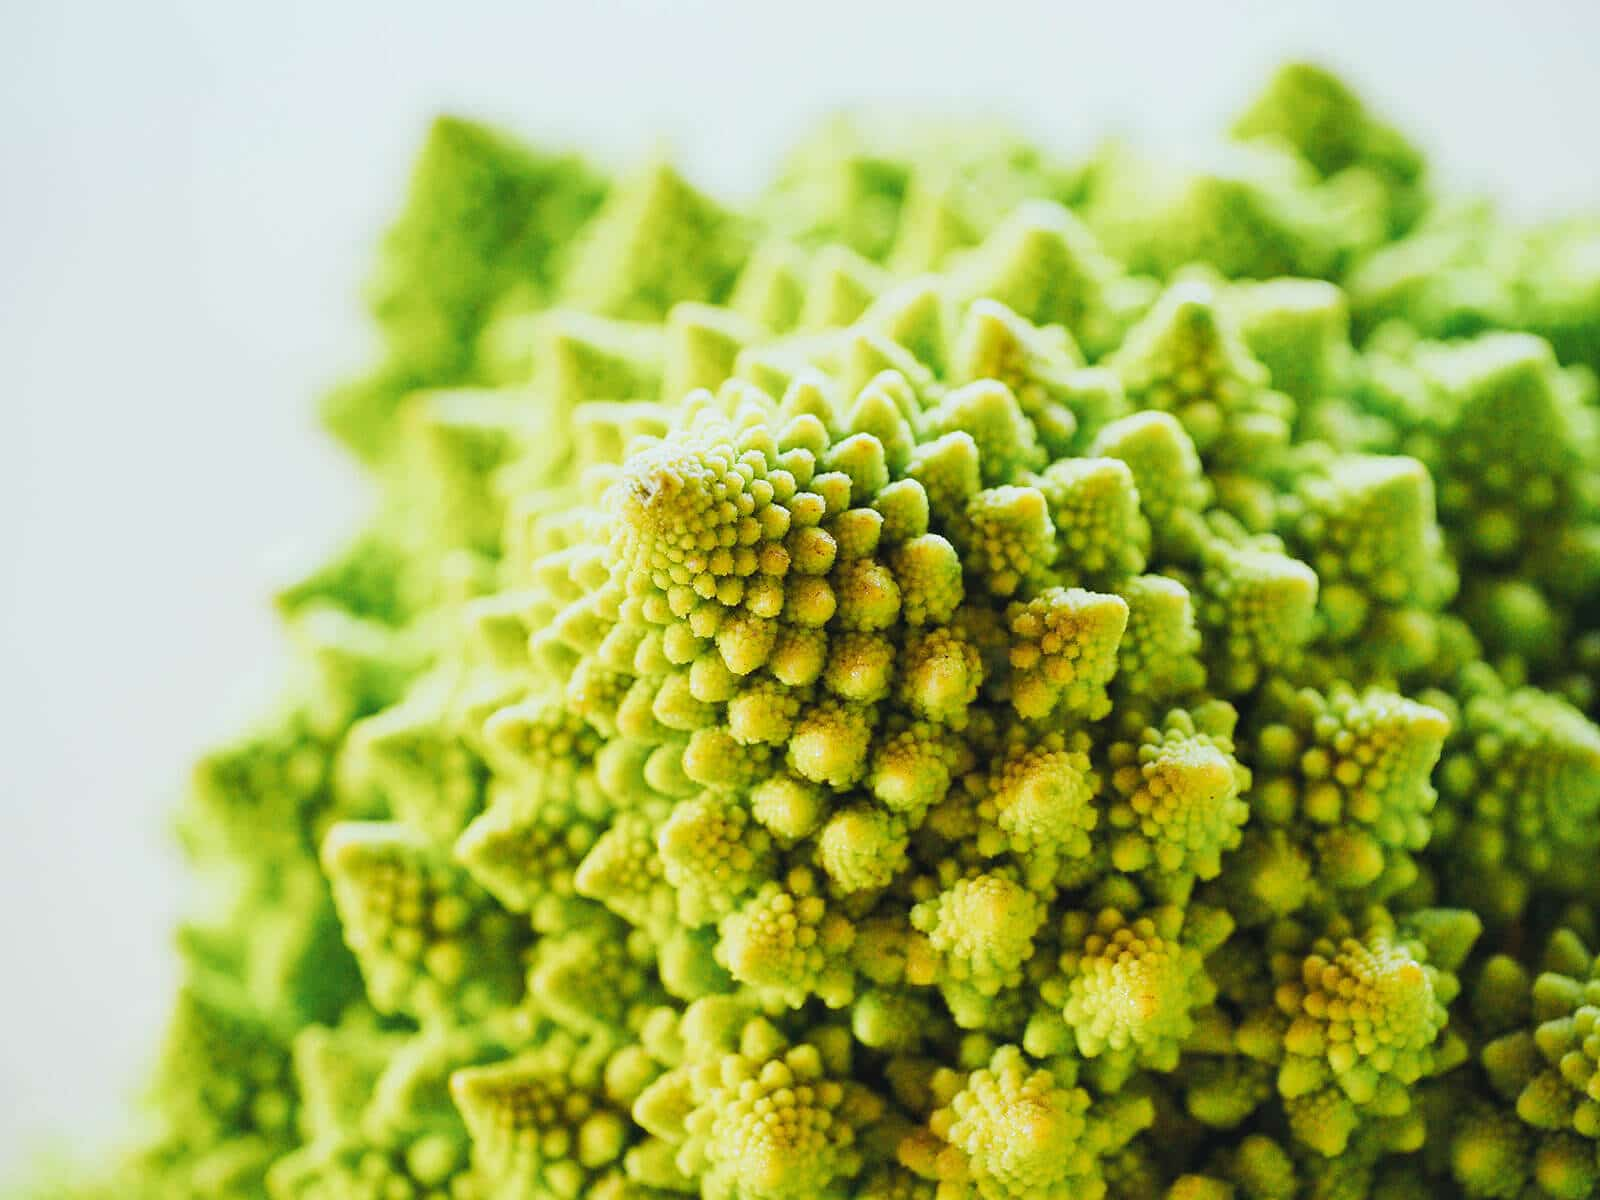
\includegraphics[width=\textwidth]{Cauliflower1.jpg}
                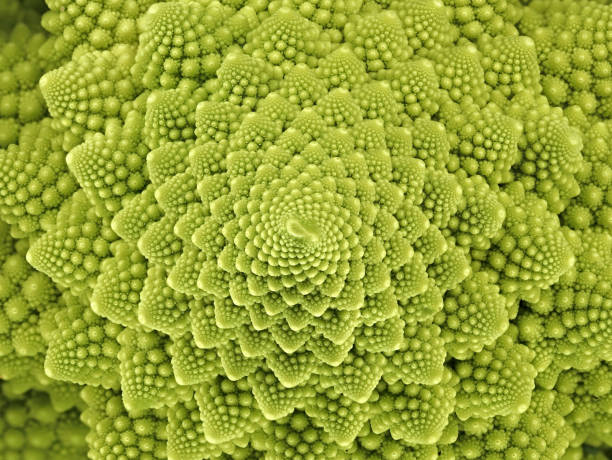
\includegraphics[width=\textwidth]{Cauliflower.jpg}
                \caption{Cauliflower from far (top) and up close (bottom).}
                \label{fig:Cauliflower}
            \end{subfigure} 
            \hfill
            % Mandelbrot images
            \begin{subfigure}[b]{0.47\textwidth}
                \centering
                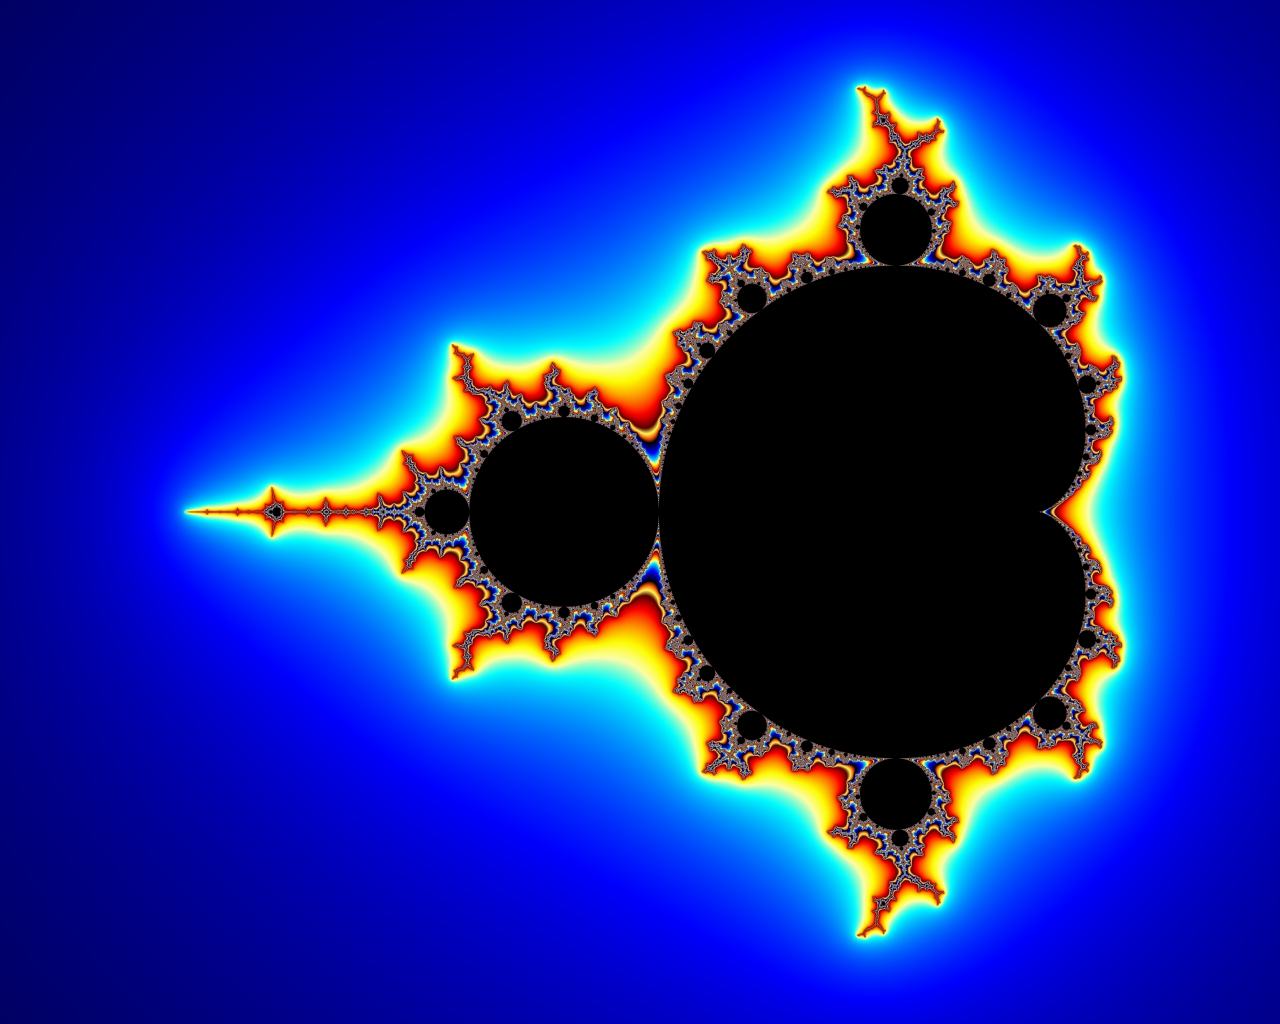
\includegraphics[width=\textwidth]{Mandelbrot_far.jpg}
                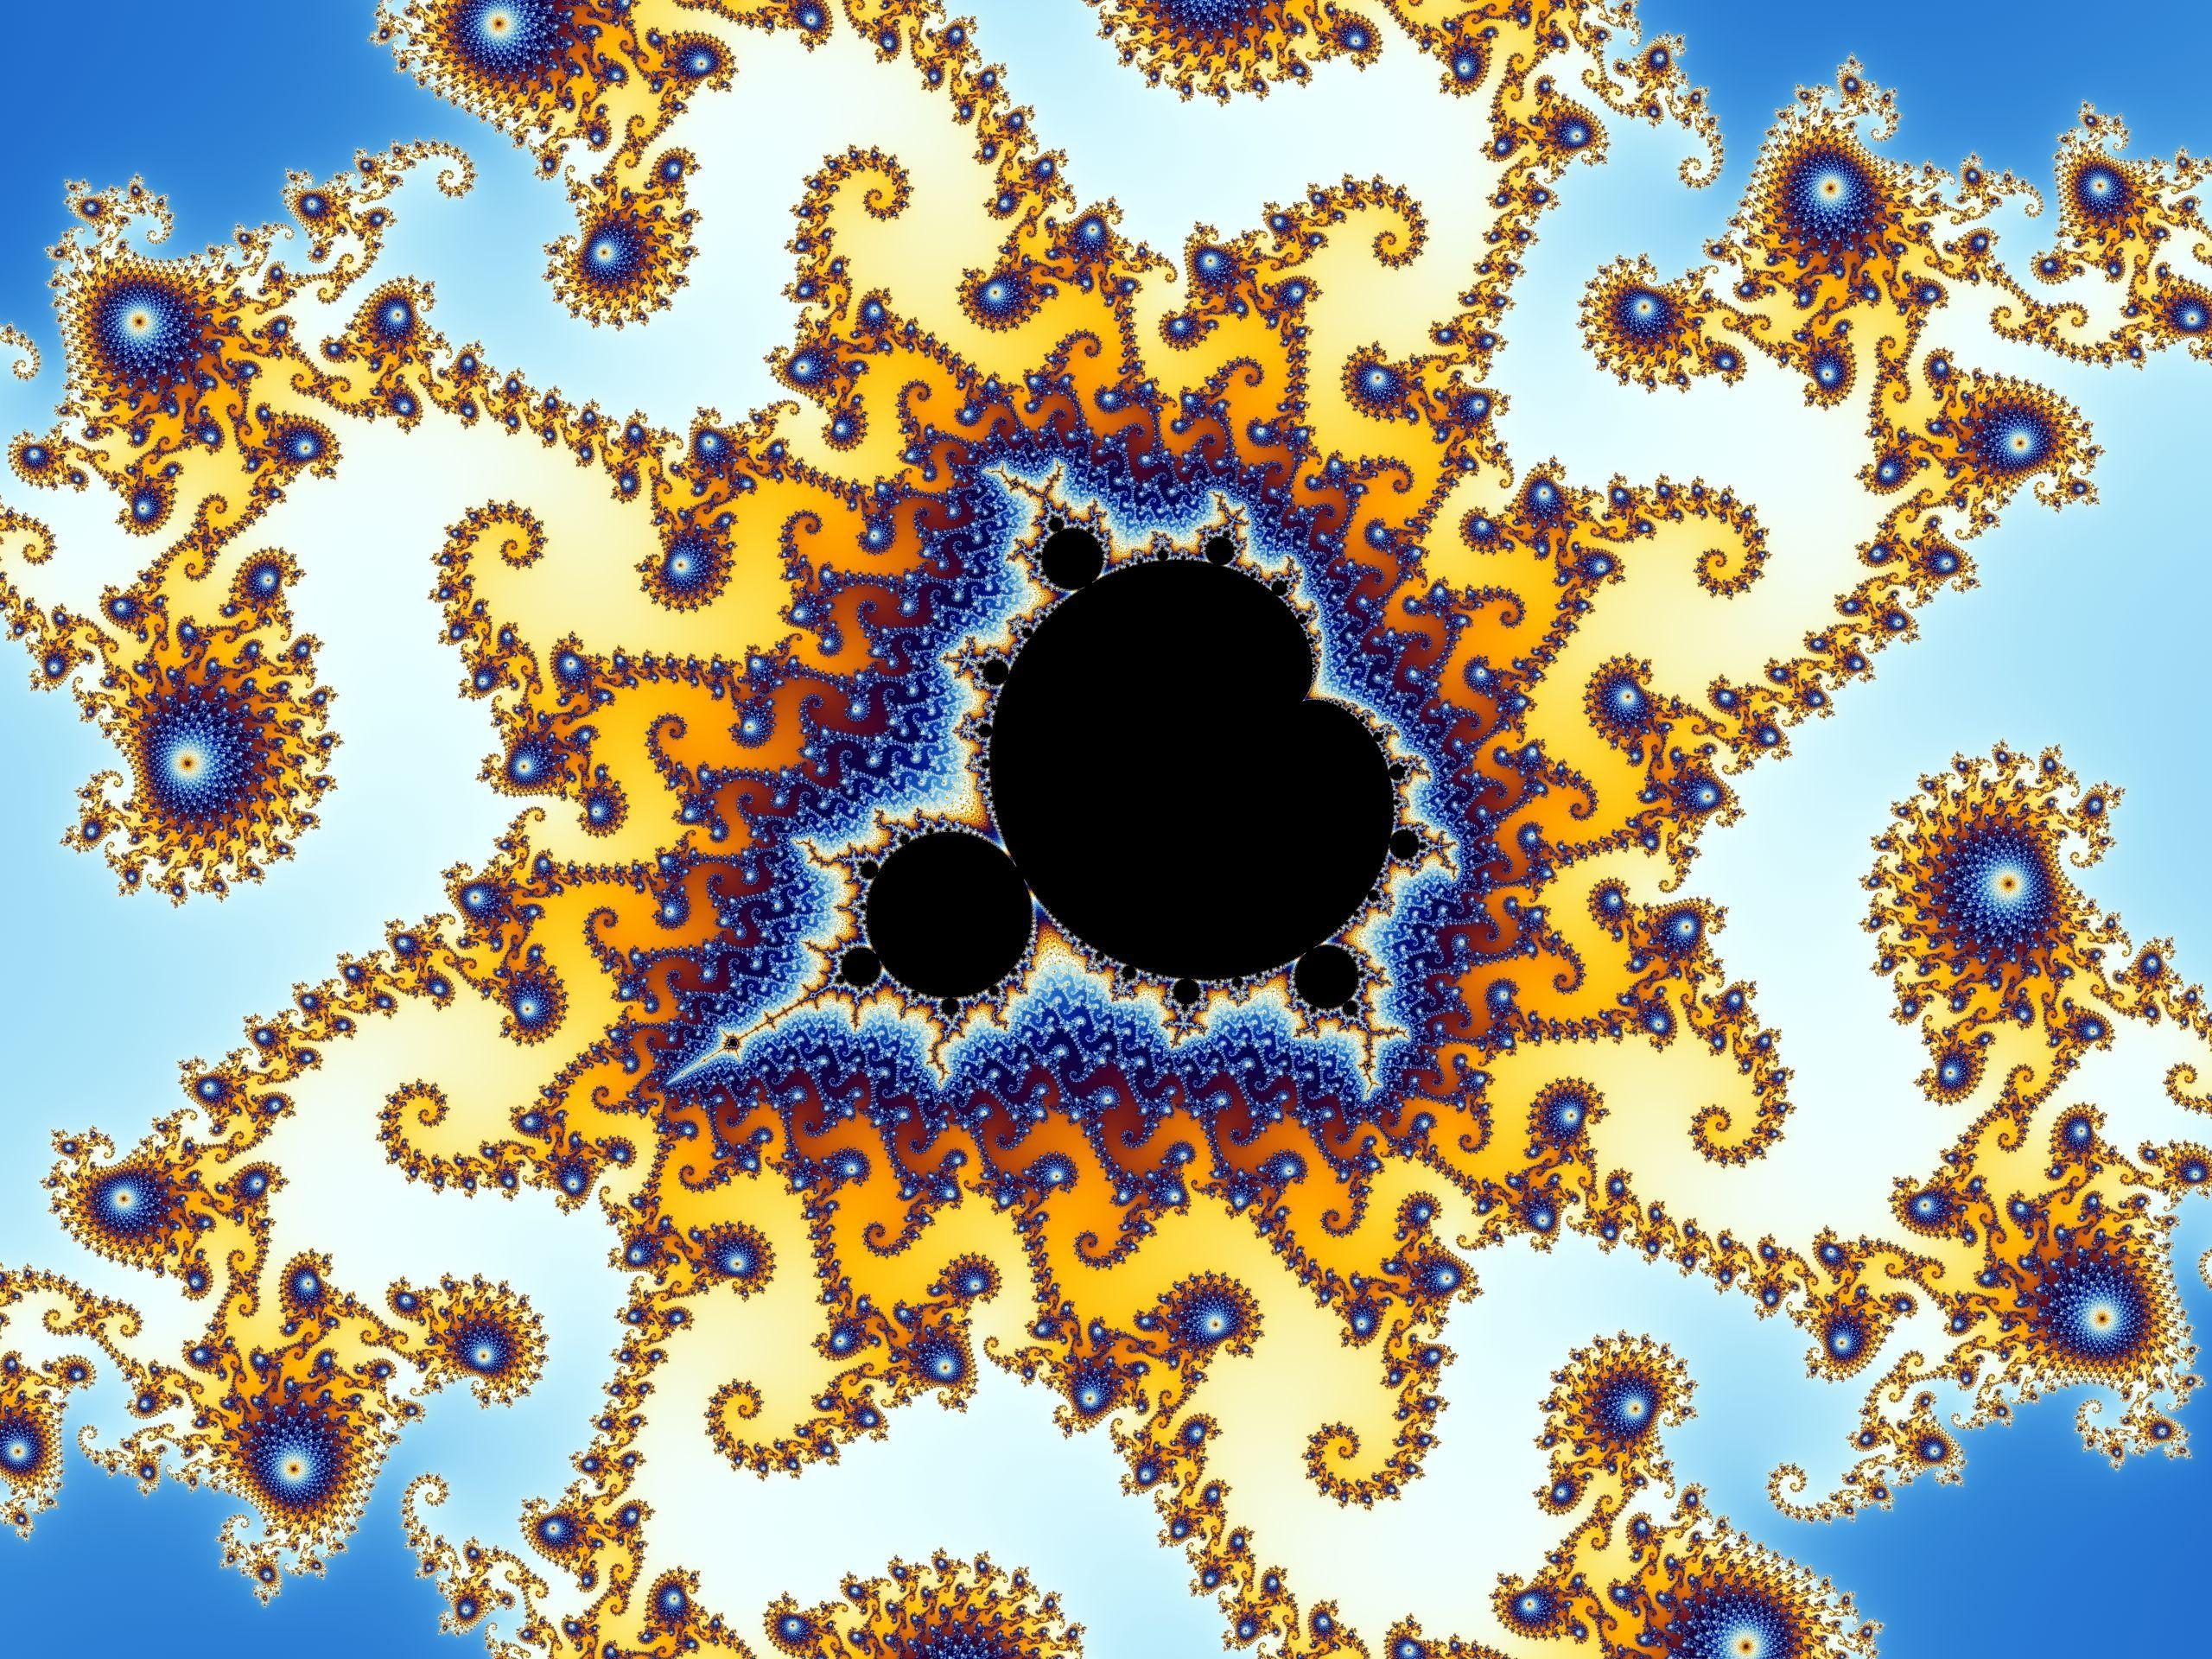
\includegraphics[width=\textwidth]{Mandelbrot_close.jpg}
                \caption{Mandelbrot set from far (top) and up close (bottom).}
                \label{fig:Mandelbrot}
            \end{subfigure}
            
        \end{minipage}%
    }
\end{figure}

\par We can observe the same level of complexity of the images as seen from far away 
and up close in figure (\ref{fig:Cauliflower}) and figure (\ref{fig:Mandelbrot}) above.

\par From a mathematical point of view, define a fractal from its changes 
in terms of mass and volume. We start from an object that we know: a square sheet 
of paper. In this case we will have the mass distributed following the area of 
the sheet, furthermore the mass grows as the square of the typical lenght of the 
sheet (the side of the square which we will call $r$). The formula will be the 
following 
\[ M = C r^2 \]
where $C$ is the surface density of the material of the sheet. We can say that the 
dimension on the sheet of paper is equal to the exponent $2$.

We can repeat the same reasoning with a metal cube, obtaining ultimately the formula
\[ M = D r^3 \]
where $D$ is the volume density of the metal used. It has of course $3$ dimensions.

\par Now let's apply this method to our experiment. Since the physical data which we 
will obtain will be the mass and the linear dimension of the system 
(the tin foil ball), the unknown parameters will be the general density $k$ and 
the dimensionality exponent $\alpha$ in the formula
\begin{equation} 
    M_{\text{experimental}} = k r_{\text{experimental}}^{\alpha}
    \label{eq:gen_fractal}
\end{equation}   

To sum up, in the following experiment we will see that also a rolled up ball of 
tin foil can be considered as a fractal.


% Materials and Methods (Tools and Procedure)
\section{Materials and Methods}
\subsection{Equipment and Tools}
\begin{itemize}
    \item Precision balance
    \item Caliber
    \item Micrometer
    \item Drawing rule and square
    \item Scissors
    \item Aluminum foil
\end{itemize}

\subsection{Experimental Procedure}
We begin by checking that we have everything at our disposal. In order to do so, we set up the laboratory as shown in Fig. (\ref{fig:lab_instr}).
Then we start off from the aluminum foil and we cut, using the scissors, a few square sheets of tin foil. 
We have to be careful in cutting squares as perfect as possible in order to reduce the error in 
the measurementes; to do so, we make use of both the ruler and the square. We cut squares of linear 
dimensions of $2 mm$, $5 mm$, $8 mm$, $11 mm$, $14 mm$, $17 mm$, $20 mm$, $23 mm$, $26 mm$ and $29 mm$.

\begin{figure}[h]
    \centering
    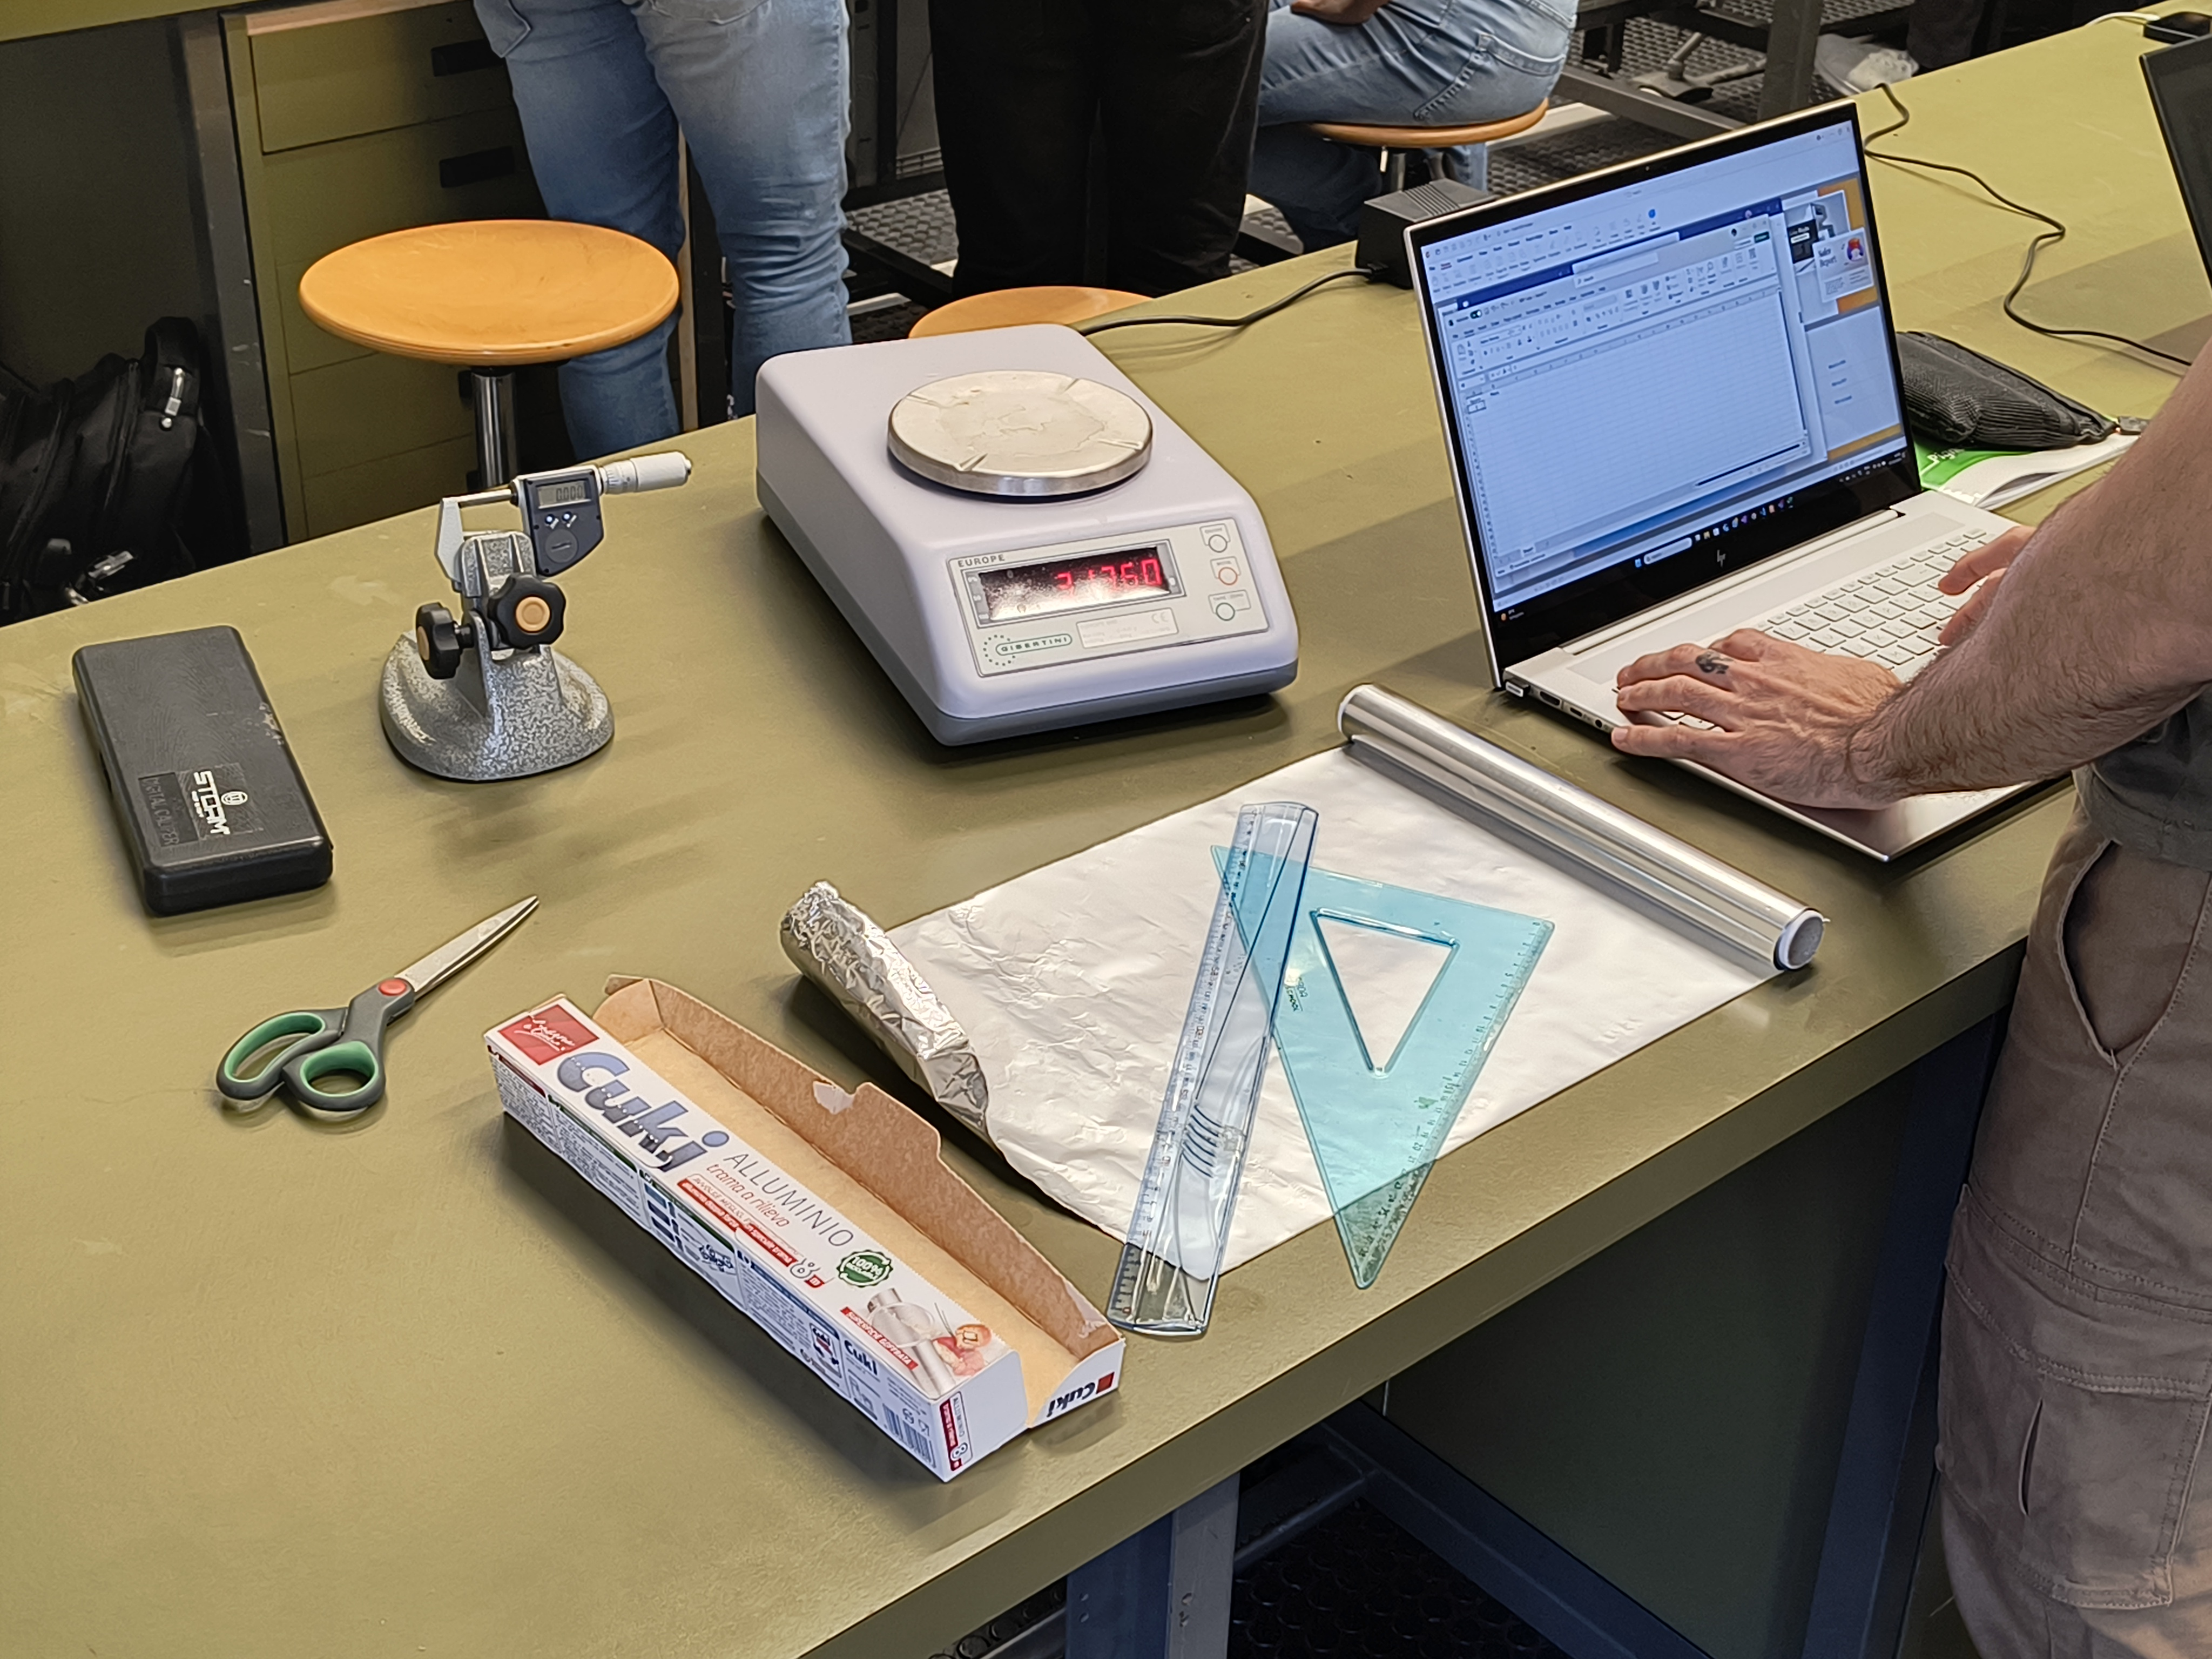
\includegraphics[width = 0.55\textwidth]{Lab_instruments.jpg}
    \caption{Our laboratory setup}
    \label{fig:lab_instr}
\end{figure}

Next, for each square, we measure the mass three times using the precision balance. We also make measurements of the different 
lenghts of the square as represented in Fig (\ref{fig:sq_measure}). Finally, we collect all data in an excel spreadsheet which we show in the next section.
\begin{figure}[h]
    \centering
    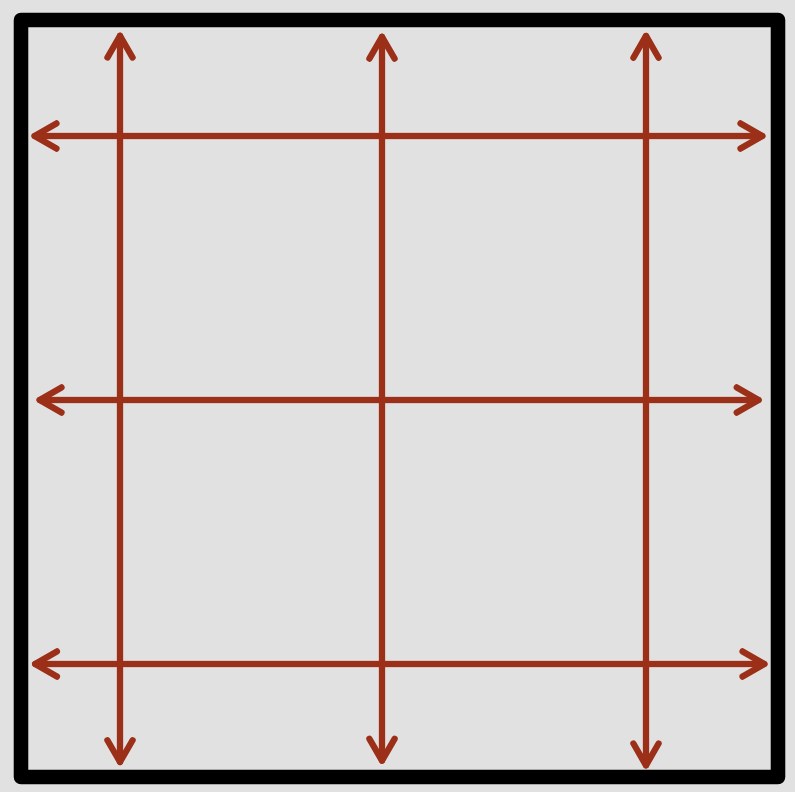
\includegraphics[width = 0.35\textwidth]{square_measure.png}
    \caption{All the direction in which we measured the lenght of the side of the aluminum foil squares} 
    \label{fig:sq_measure}
\end{figure}

Now, we roll up every tin foil square into a sphere trying to have each ball at the same density as shown in Fig. (\ref{fig:tf_balls}). 
Since we do this operation by hand, we can only have an idea of its density. This is the step in the 
procedure which, according to us, correspond to the biggest source of error in the experiment.

\begin{figure}[h]
    \centering
    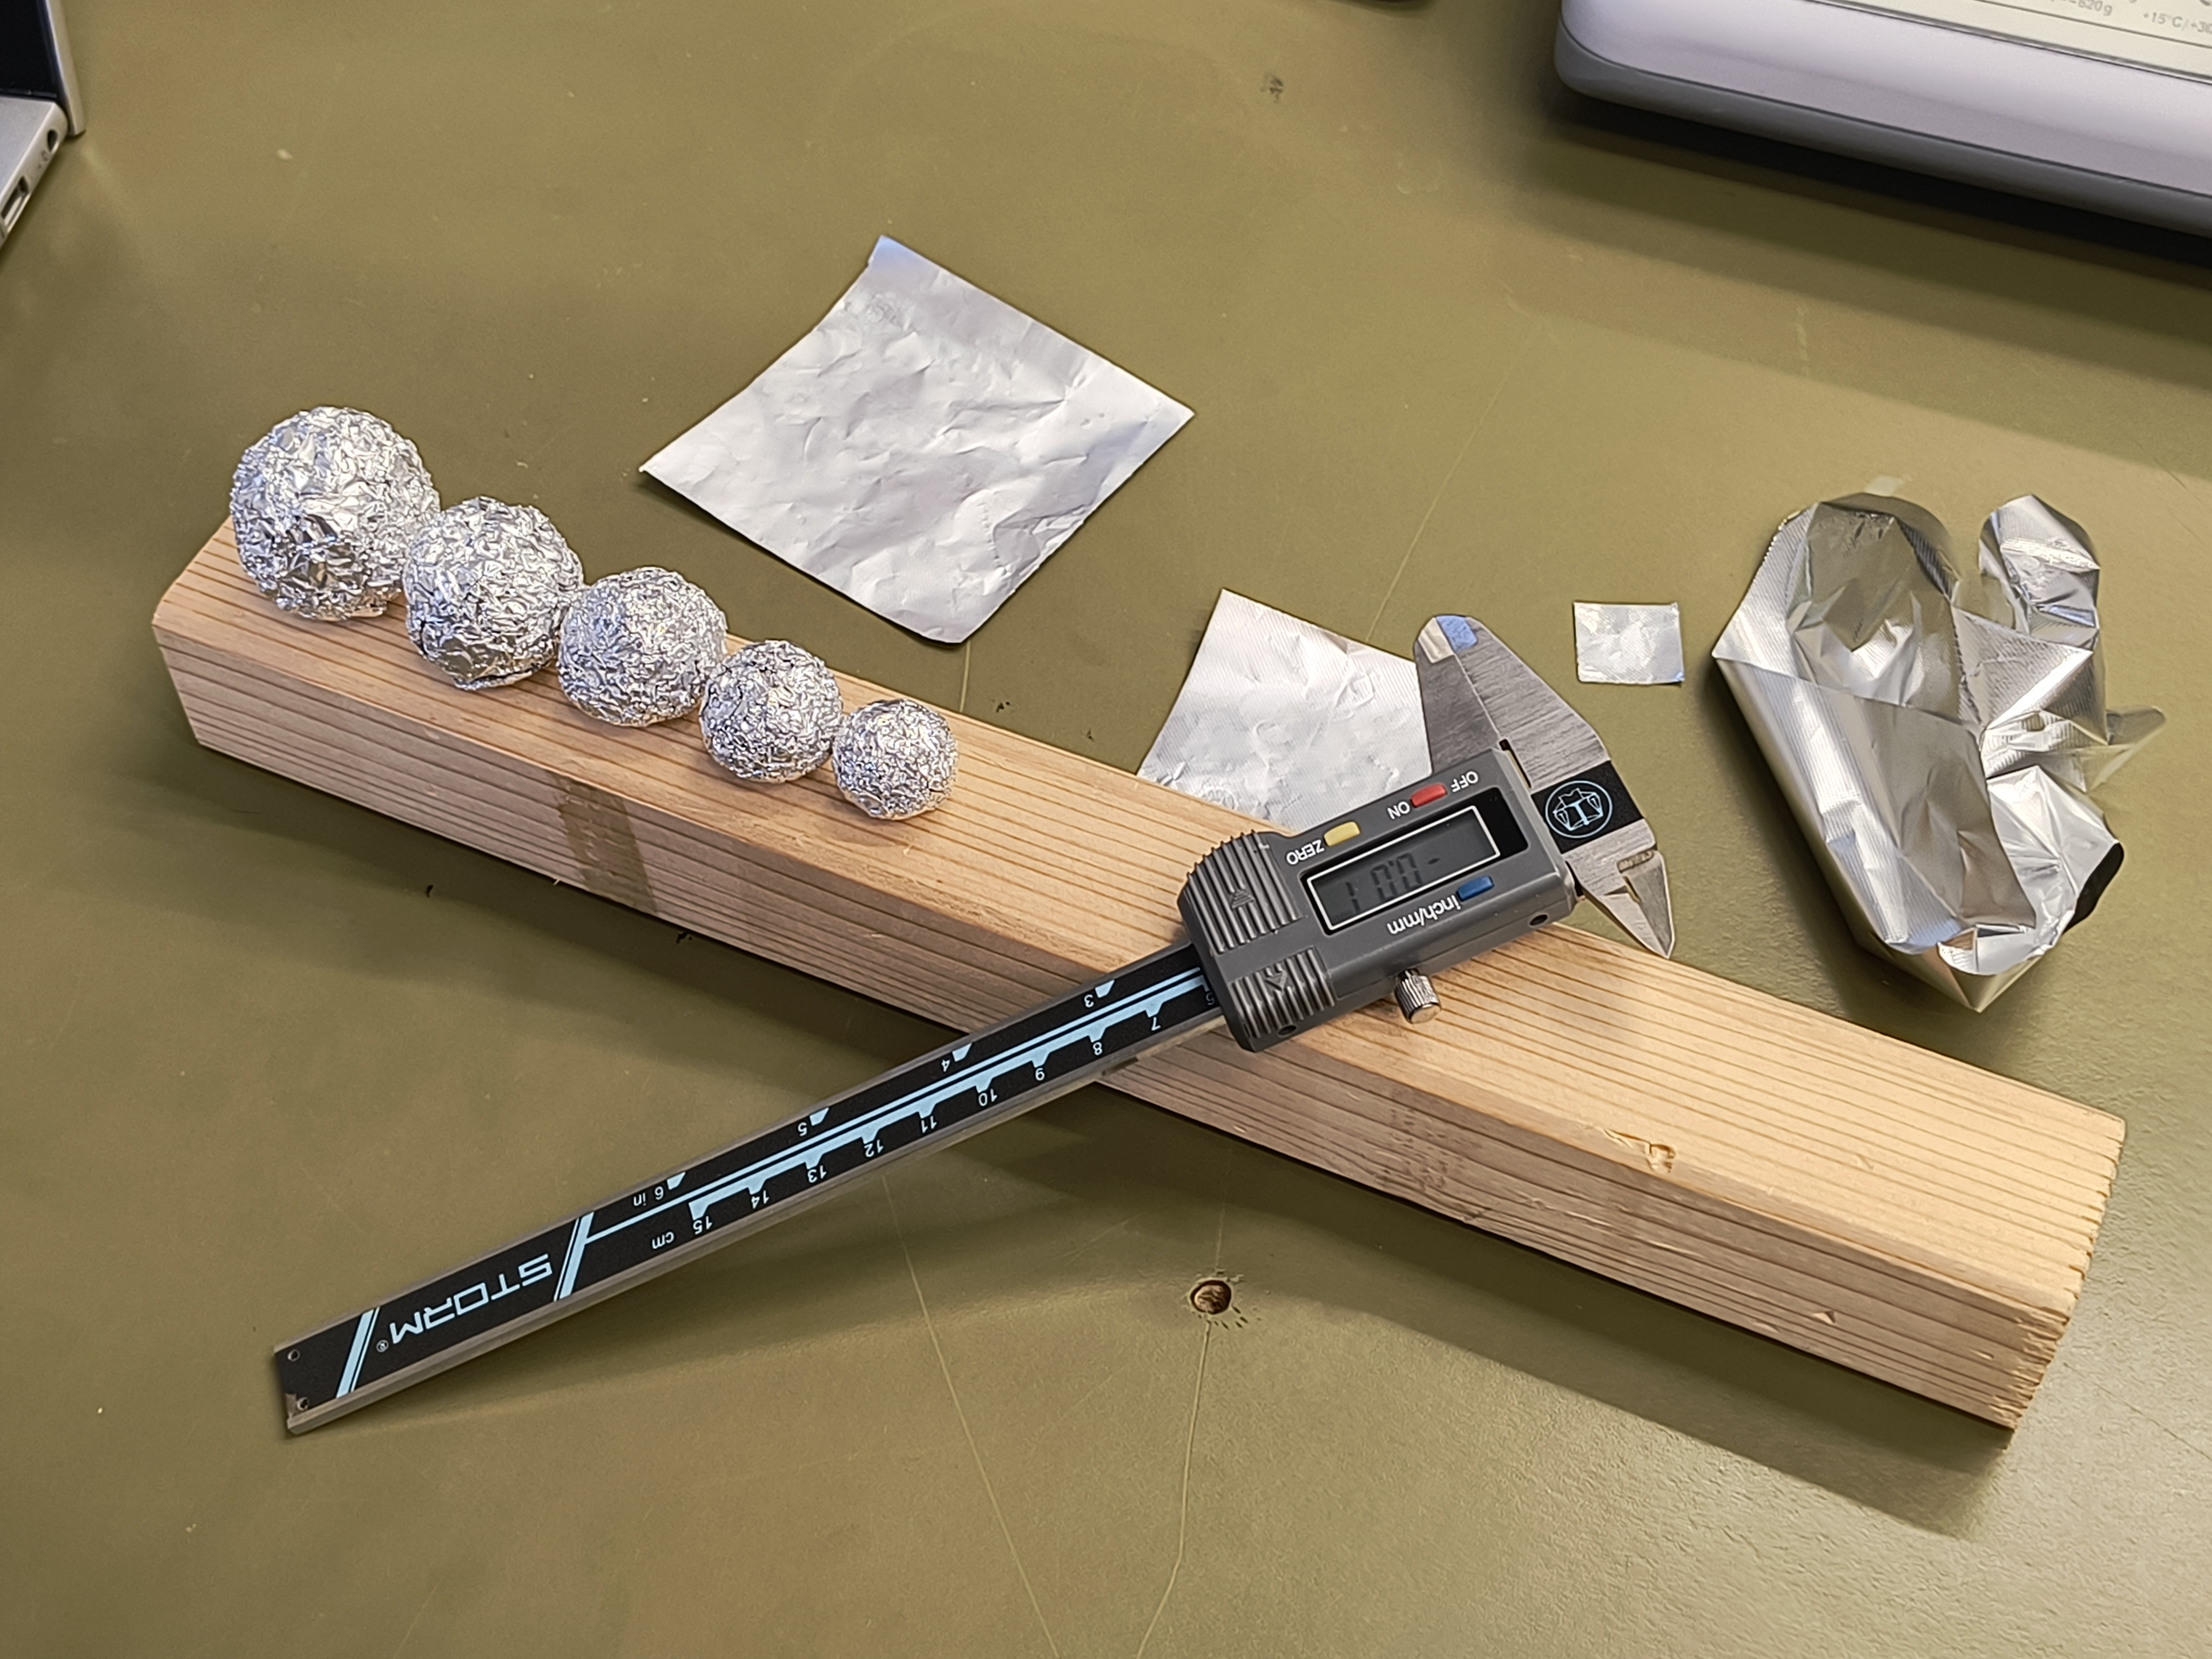
\includegraphics[width = 0.55\textwidth]{Tin_foil_balls.jpg}
    \caption{Some of the balls that me made from the tin foil, the caliber, some squares of tin foil in the background}
    \label{fig:tf_balls}
\end{figure}

Once finished, our last measurent was to collect the information of the linear dimension (its diameter) 
of each ball. We use the caliber or the micrometer (depending on the size of the ball) to measure the diameter 
of the ball along three different axis. We put this data in an excel spreadsheet too.

% Results (Graphs and Data)
\section{Results}\label{sec:results}
\subsection{Part 1: Aluminum Foil Squares}
The data collected from the aluminum foil squares is shown in Tables (\ref{tab:squares}) and (\ref{tab:balls}); for instance, as explained in the preceding section, 
for each square, we measured six times its linear dimension along different axis in order to reduce the error in the measurements. 
In the same way, while measuring the mass of the squares, we repeated the same procedure three times and the related data is shown 
in Table (\ref{tab:balls}).

\begin{table}[!ht]
    \centering
    \begin{tabular}{|c|c|c|c|}
    \hline
        \textbf{Square (cm)} & \( \overline{L} \pm \Delta L \) (cm) & \( \overline{m} \pm \Delta m \) (g) \\ \hline 
        \textbf{29x29} & 29.02 \(\pm\) 0.11 & 2.80 \(\pm\) 0.012 \\ \hline
        \textbf{26x26} & 26.02 \(\pm\) 0.13 & 2.28 \(\pm\) 0.010 \\ \hline
        \textbf{23x23} & 23.00 \(\pm\) 0.10 & 1.77 \(\pm\) 0.010 \\ \hline 
        \textbf{20x20} & 20.02 \(\pm\) 0.11 & 1.34 \(\pm\) 0.010 \\ \hline
        \textbf{17x17} & 17.02 \(\pm\) 0.11 & 0.97 \(\pm\) 0.010 \\ \hline
        \textbf{14x14} & 14.00 \(\pm\) 0.12 & 0.66 \(\pm\) 0.010 \\ \hline
        \textbf{11x11} & 11.00 \(\pm\) 0.10 & 0.40 \(\pm\) 0.010 \\ \hline
        \textbf{8x8}   & 7.98  \(\pm\) 0.11 & 0.21 \(\pm\) 0.010 \\ \hline
        \textbf{5x5}   & 5.00  \(\pm\) 0.10 & 0.08 \(\pm\) 0.010 \\ \hline
    \end{tabular}
    \caption{Measurements of Squares with Average Length and Mass with their respective uncertainties}
    \label{tab:squares}
\end{table}



\subsection{Part 2: Crumpled Aluminum folis}
\begin{table}[h!] 
    \centering
    \begin{tabular}{|c|c|c|c|}
    \hline
        \textbf{Square (cm)} & \( \overline{D} \pm \Delta D \) (mm) \\ \hline 
        \textbf{29x29} & 35.348 \(\pm\) 0.903              \\ \hline
        \textbf{26x26} & 29.245 \(\pm\) 0.881              \\ \hline
        \textbf{23x23} & 25.852 \(\pm\) 0.327              \\ \hline
        \textbf{20x20} & 23.304 \(\pm\) 1.319              \\ \hline
        \textbf{17x17} & 20.240 \(\pm\) 1.177              \\ \hline
        \textbf{14x14} & 18.170 \(\pm\) 0.720              \\ \hline
        \textbf{11x11} & 14.950 \(\pm\) 0.824              \\ \hline
        \textbf{8x8}   & 10.643 \(\pm\) 0.386              \\ \hline
        \textbf{5x5}   & 7.535  \(\pm\) 0.305              \\ \hline
        \textbf{3x3}   & 3.117 \(\pm\) 0.212               \\ \hline
    \end{tabular}
    \caption{Diameters values for each aluminum ball with their respective uncertainties}
    \label{tab:balls}
\end{table}

For the second part of the experiment, after having rolled up all the squares into balls, we proceded to measure each diameter as explained in the previous section. The data collected from this measurements is reported in Table (\ref{tab:balls}).




\subsection{Remarks on the Data processing} 
We also compute the natural logarithm of the mean values of the mass, the diameter and the lenght shown in the tables above. The related errors are calculated using traditional methods of error propagation \cite{taylor-1997}, having taking into account the uncertainties of both casual and systematic nature. The results are shown in Table (\ref{tab:ln_errors}). These quantities will be useful in the following sections for the computation of the fractal dimension of the system using the well known Least Squares method.


\begin{table}[!ht]
    \centering
    \begin{tabular}{|c|c|c|c|c|c|}
    \hline
        \( \ln(L) \pm \Delta \ln(L) \) & \( \ln(m) \pm \Delta \ln(m) \) & \( \ln(D) \pm \Delta \ln(D) \) \\ \hline
        3.368 \(\pm\) 0.004 & 1.028 \(\pm\) 0.004 & 3.565 \(\pm\) 0.253 \\ \hline
        3.259 \(\pm\) 0.005 & 0.824 \(\pm\) 0.004 & 3.376 \(\pm\) 0.261 \\ \hline
        3.135 \(\pm\) 0.004 & 0.571 \(\pm\) 0.006 & 3.252 \(\pm\) 0.100 \\ \hline
        2.997 \(\pm\) 0.005 & 0.293 \(\pm\) 0.007 & 3.149 \(\pm\) 0.419 \\ \hline
        2.834 \(\pm\) 0.006 & -0.030 \(\pm\) 0.010 & 3.008 \(\pm\) 0.391 \\ \hline
        2.639 \(\pm\) 0.008 & -0.416 \(\pm\) 0.015 & 2.900 \(\pm\) 0.248 \\ \hline
        2.398 \(\pm\) 0.009 & -0.916 \(\pm\) 0.025 & 2.705 \(\pm\) 0.305 \\ \hline
        2.077 \(\pm\) 0.014 & -1.561 \(\pm\) 0.048 & 2.365 \(\pm\) 0.163 \\ \hline
        1.609 \(\pm\) 0.020 & -2.526 \(\pm\) 0.125 & 2.020 \(\pm\) 0.151 \\ \hline
        1.099 \(\pm\) 0.033 & -3.912 \(\pm\) 0.500 & 1.137 \(\pm\) 0.187 \\ \hline
    \end{tabular}
    \caption{Natural Logarithms and Their Errors}
    \label{tab:ln_errors}
\end{table}


% Discussion and Analysis
\section{Discussion and Analysis}
\par Once the data has been fully analysed, we can start by discussing the main results obtained from the experiment. 
In particular, studying the plot shown in Fig. (\ref{fig:mass_vs_length}) which describes the relationship between the mass of the aluminum 
squares and their linear dimension, we can easily observe (as expected) that the data is well represented by a power law.

\begin{figure}[h!] 
    \centering
    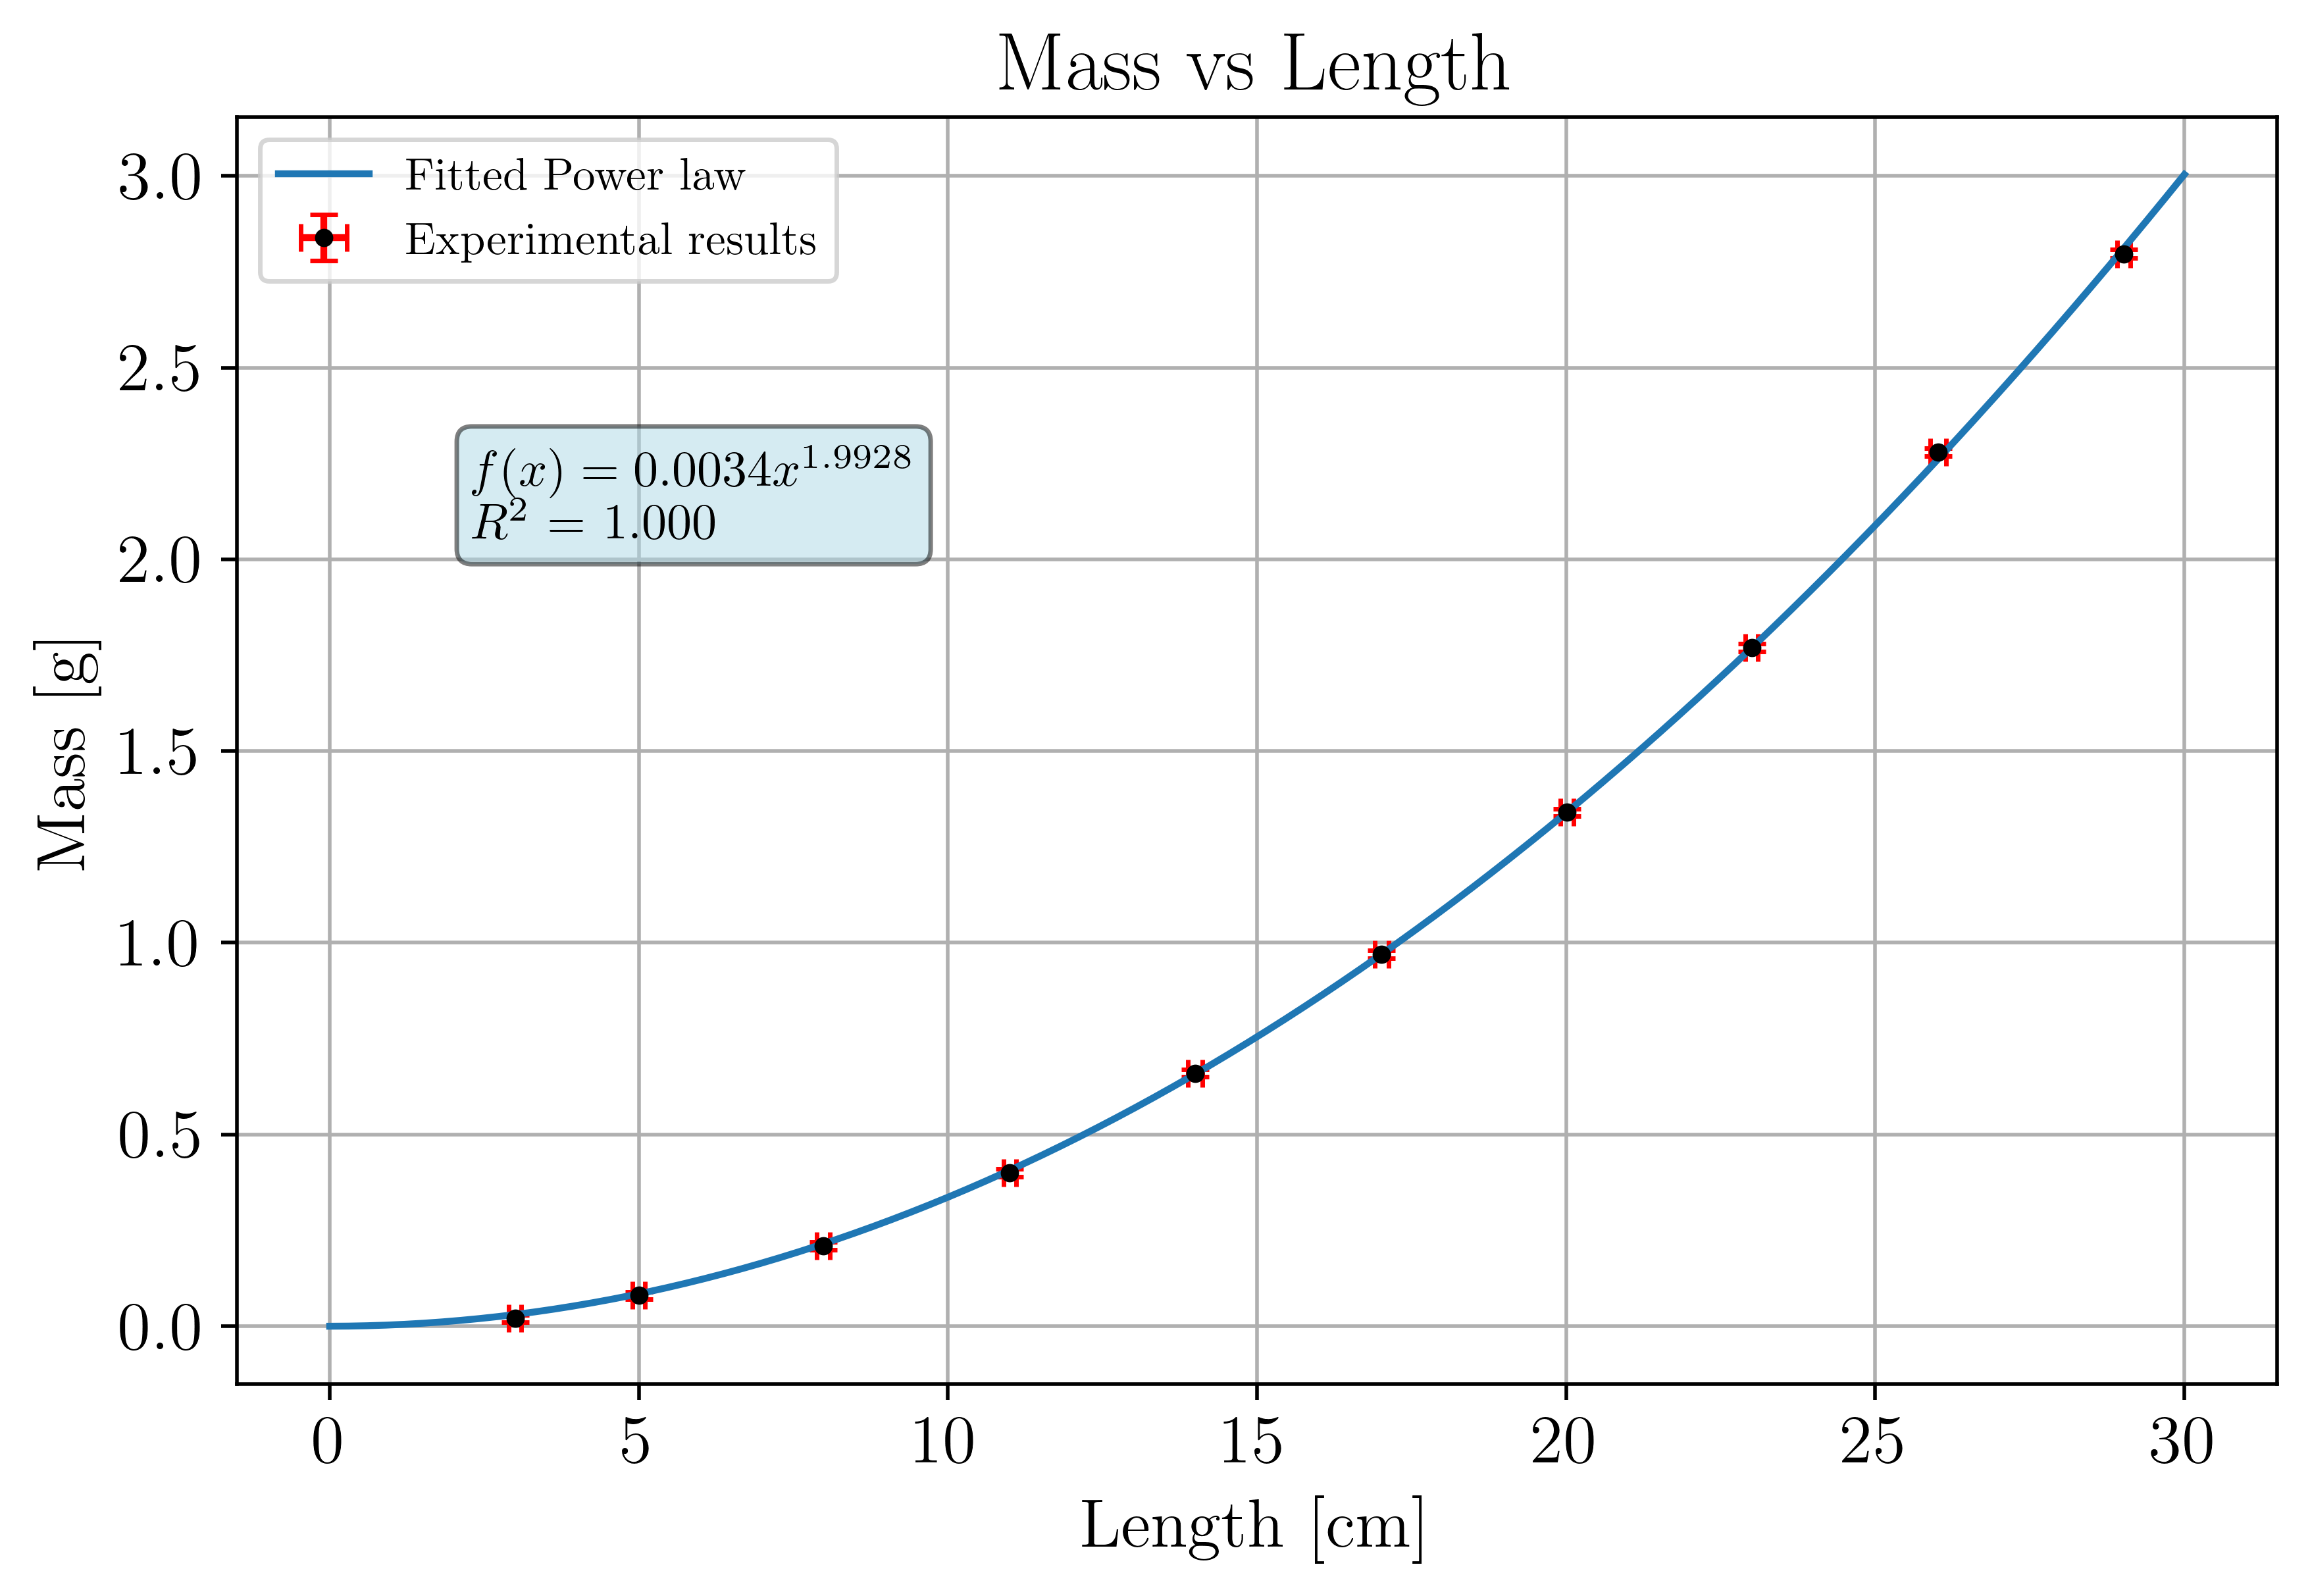
\includegraphics[width = 0.8\textwidth]{mass_vs_length.png}
    \caption{Mass vs Length of the Aluminum Squares}
    \label{fig:mass_vs_length}
\end{figure}

The power law obtained from the data is given by the the equation
\begin{equation}\label{eq:mass_vs_length}
    M = 0.0034 L^{1.9928}
\end{equation}
where $M$ corresponds to the mass of the aluminum squares and $L$ to its linear dimension. The exponent of the power law is very close to $2$, which is the expected 
value for a two-dimensional object. This law was obtained numerically using the Python library \texttt{scipy} and the function \texttt{curve\_fit} (see Appendix ref). 
This is a very satisfactory result supported by the associated $R^2$ parameter, which validates the fit of the data to the expected power law.  

In addition, we can consider a different approach to the problem by using the Least Squares method to compute both parameters of the power law. With this aim, we calculate 
the natural logarithm of the general law $M = k L^{\alpha}$, obtaining 
\begin{equation}
    \ln(M) = \ln(k) + \alpha \ln(L),
\end{equation}
which clearly describe a linear dependence between the natural logarithm of the mass and the natural logarithm of the linear dimension. Using the data from Table (\ref{tab:ln_errors}), we can plot this relationship and compute the parameters $k$ and $\alpha$ using the Least Squares method. The results are shown in Fig. (\ref{fig:ln_mass_vs_ln_length}).
\begin{figure}[h!]
    \centering
    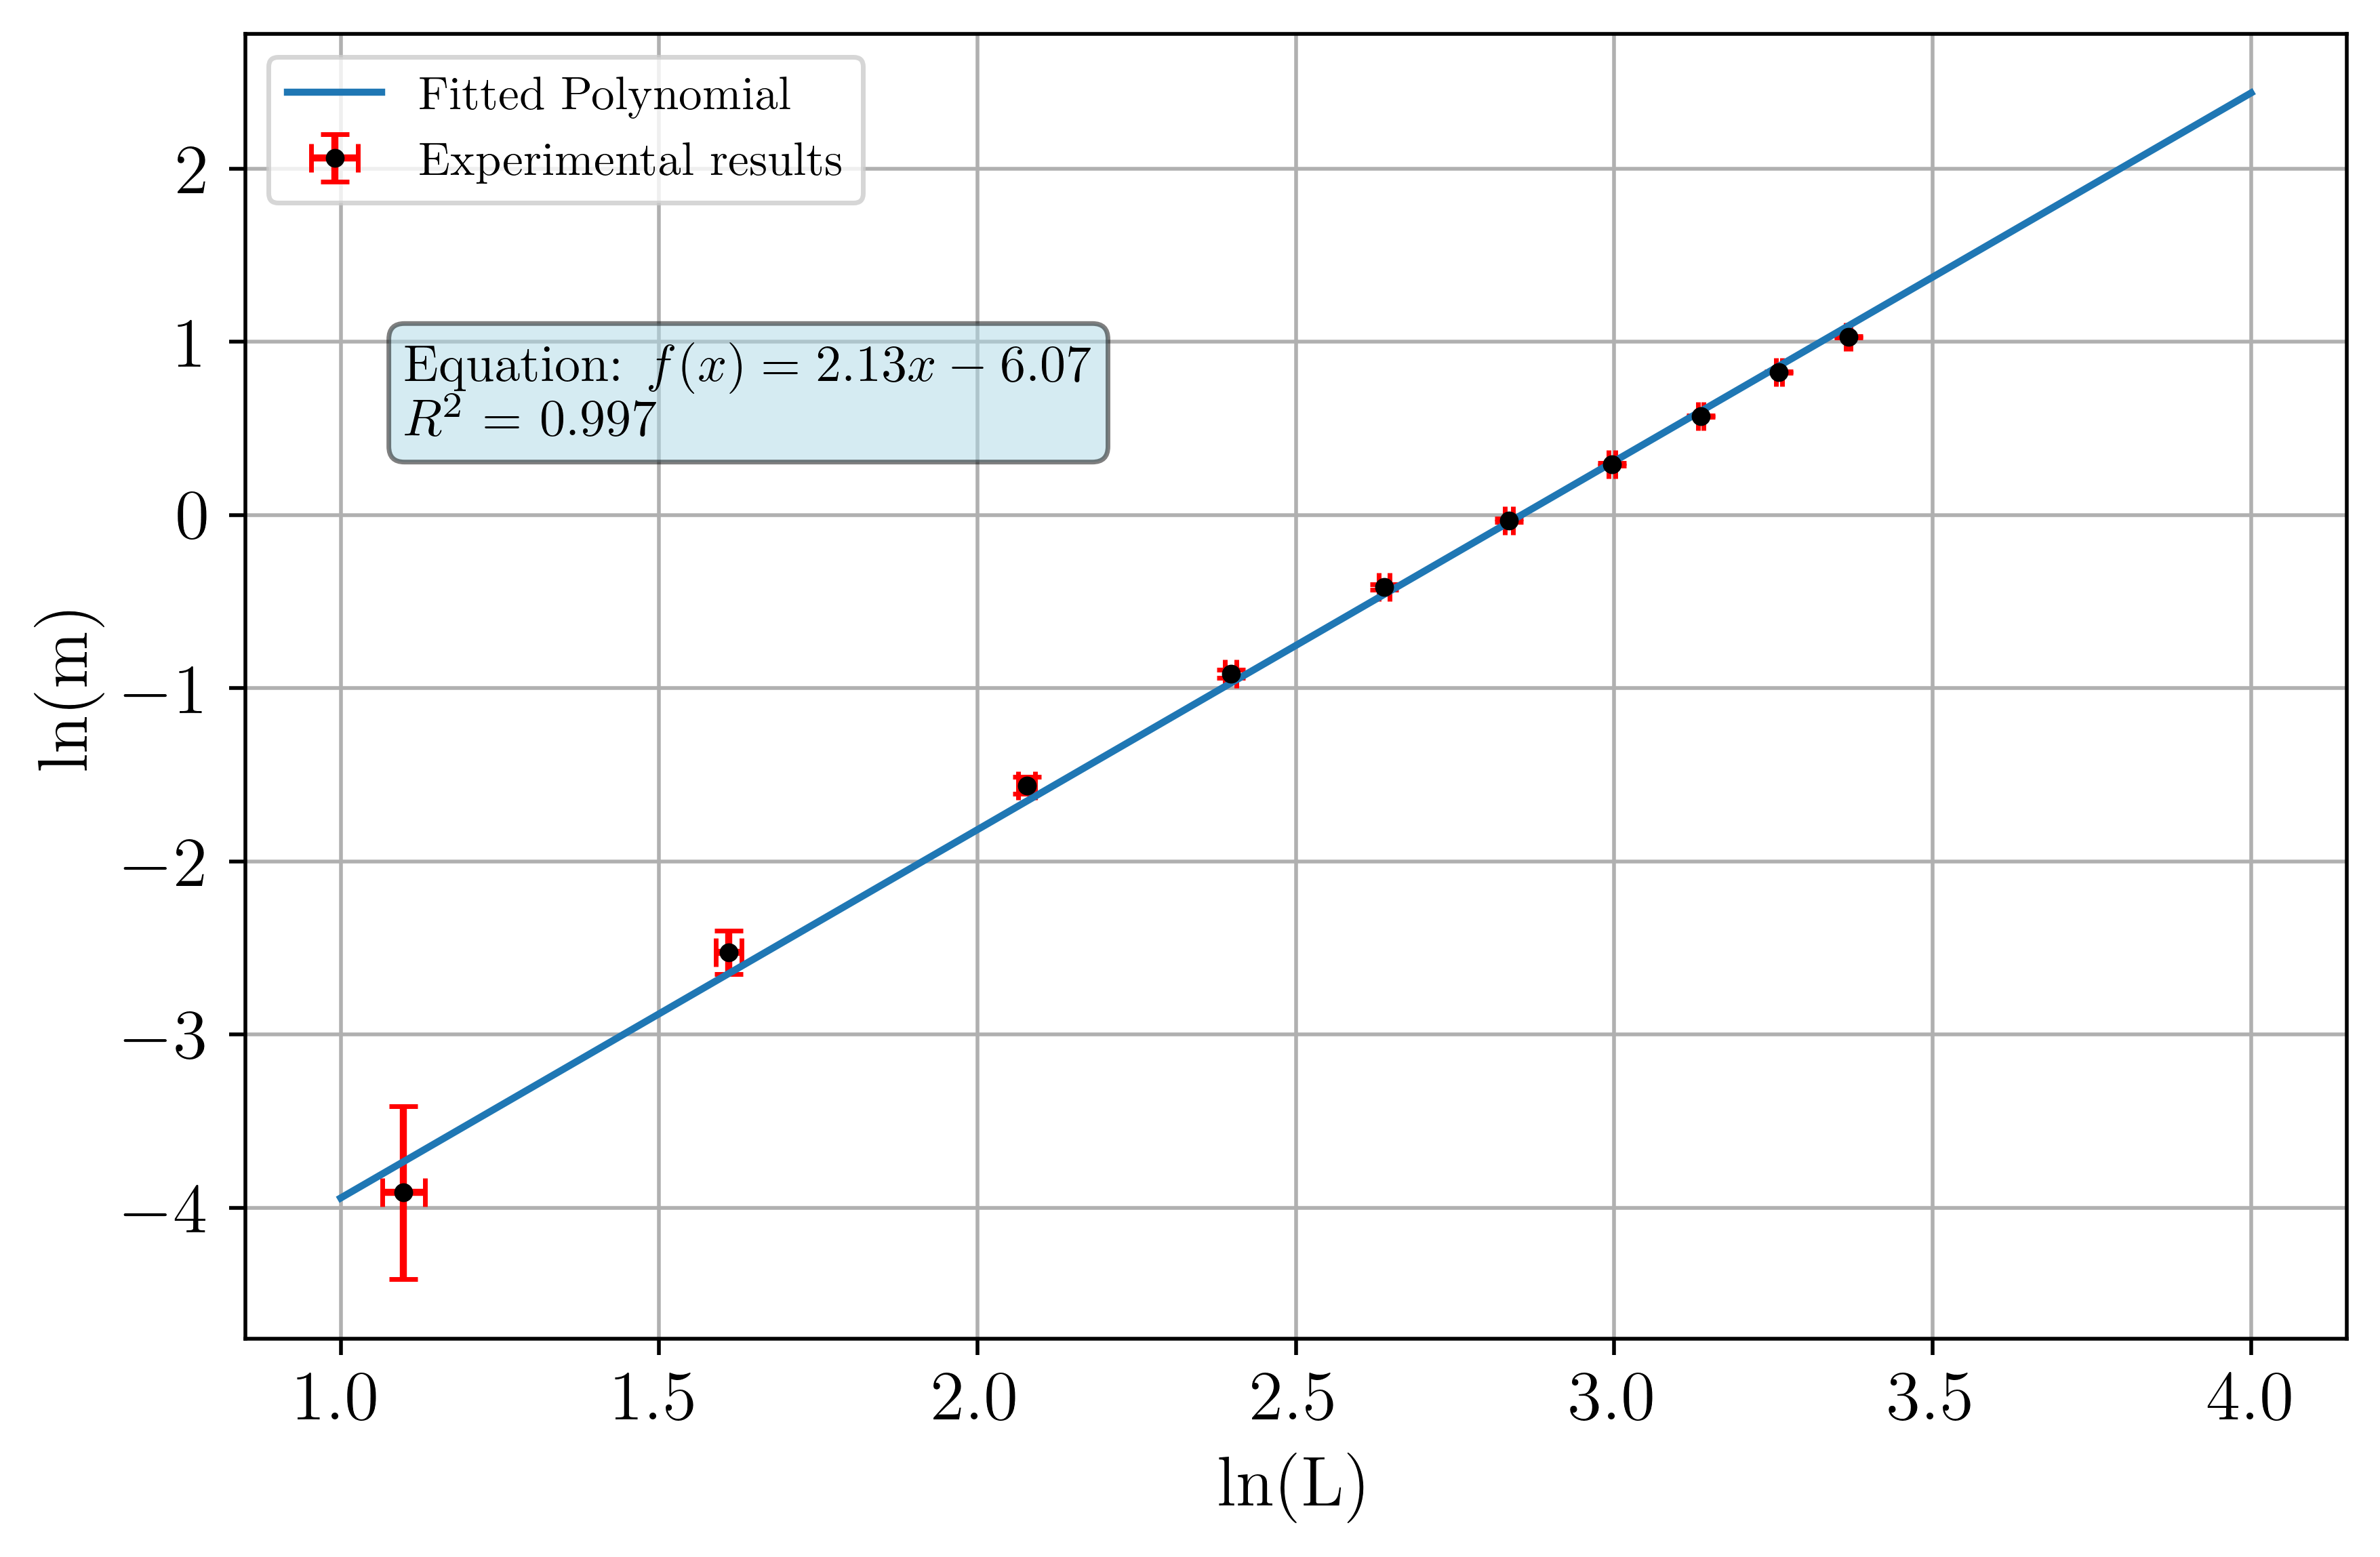
\includegraphics[width = 0.8\textwidth]{ln_mass_vs_ln_length.png}
    \caption{Natural logarithm of Mass vs Natural logarithm of Length of the Aluminum Squares. Alternative approach for the computation of the dimensionality parameters.}
    \label{fig:ln_mass_vs_ln_length}
\end{figure}

As expected, we obtained that the data is well represented by a linear function, whose parameters $\ln(k)$ and $\alpha$ correspond to the slope and the intercept of the line, respectively. The values obtained for these parameters are $\ln(k) = -6.07 \pm 0.11$ and $\alpha = 2.13 \pm  0.04$. These values are in perfect agreement with the ones obtained from the previous method, which validates the results obtained from the experiment.

On the other hand, for the second part of the experiment, we follow the same procedure as before, and now we study the relationship between the mass 
of the aluminum squares (now crumpled aluminum balls) and their linear dimension: the diameter. The plot shown in Fig. (\ref{fig:mass_vs_diameter}) 
describes this relationship and, as expected, the data is well represented by a power law. However, the exponent we obtained in this case contradicts our predictions since we expected a value ranging from $2$ to $3$. This discrepancy could be due to the fact that the balls were not perfectly rolled up, which could have affected the measurements of the diameter and consequently the results obtained from the experiment. Even if the $R^2$ parameter is very close to $1$, we can not consider the results obtained from this part of the experiment as satisfactory. In order to improve these results, one could collect more data regarding the diameter of each ball by measuring them across several more different axis. 

\begin{figure}[h!]
    \centering
    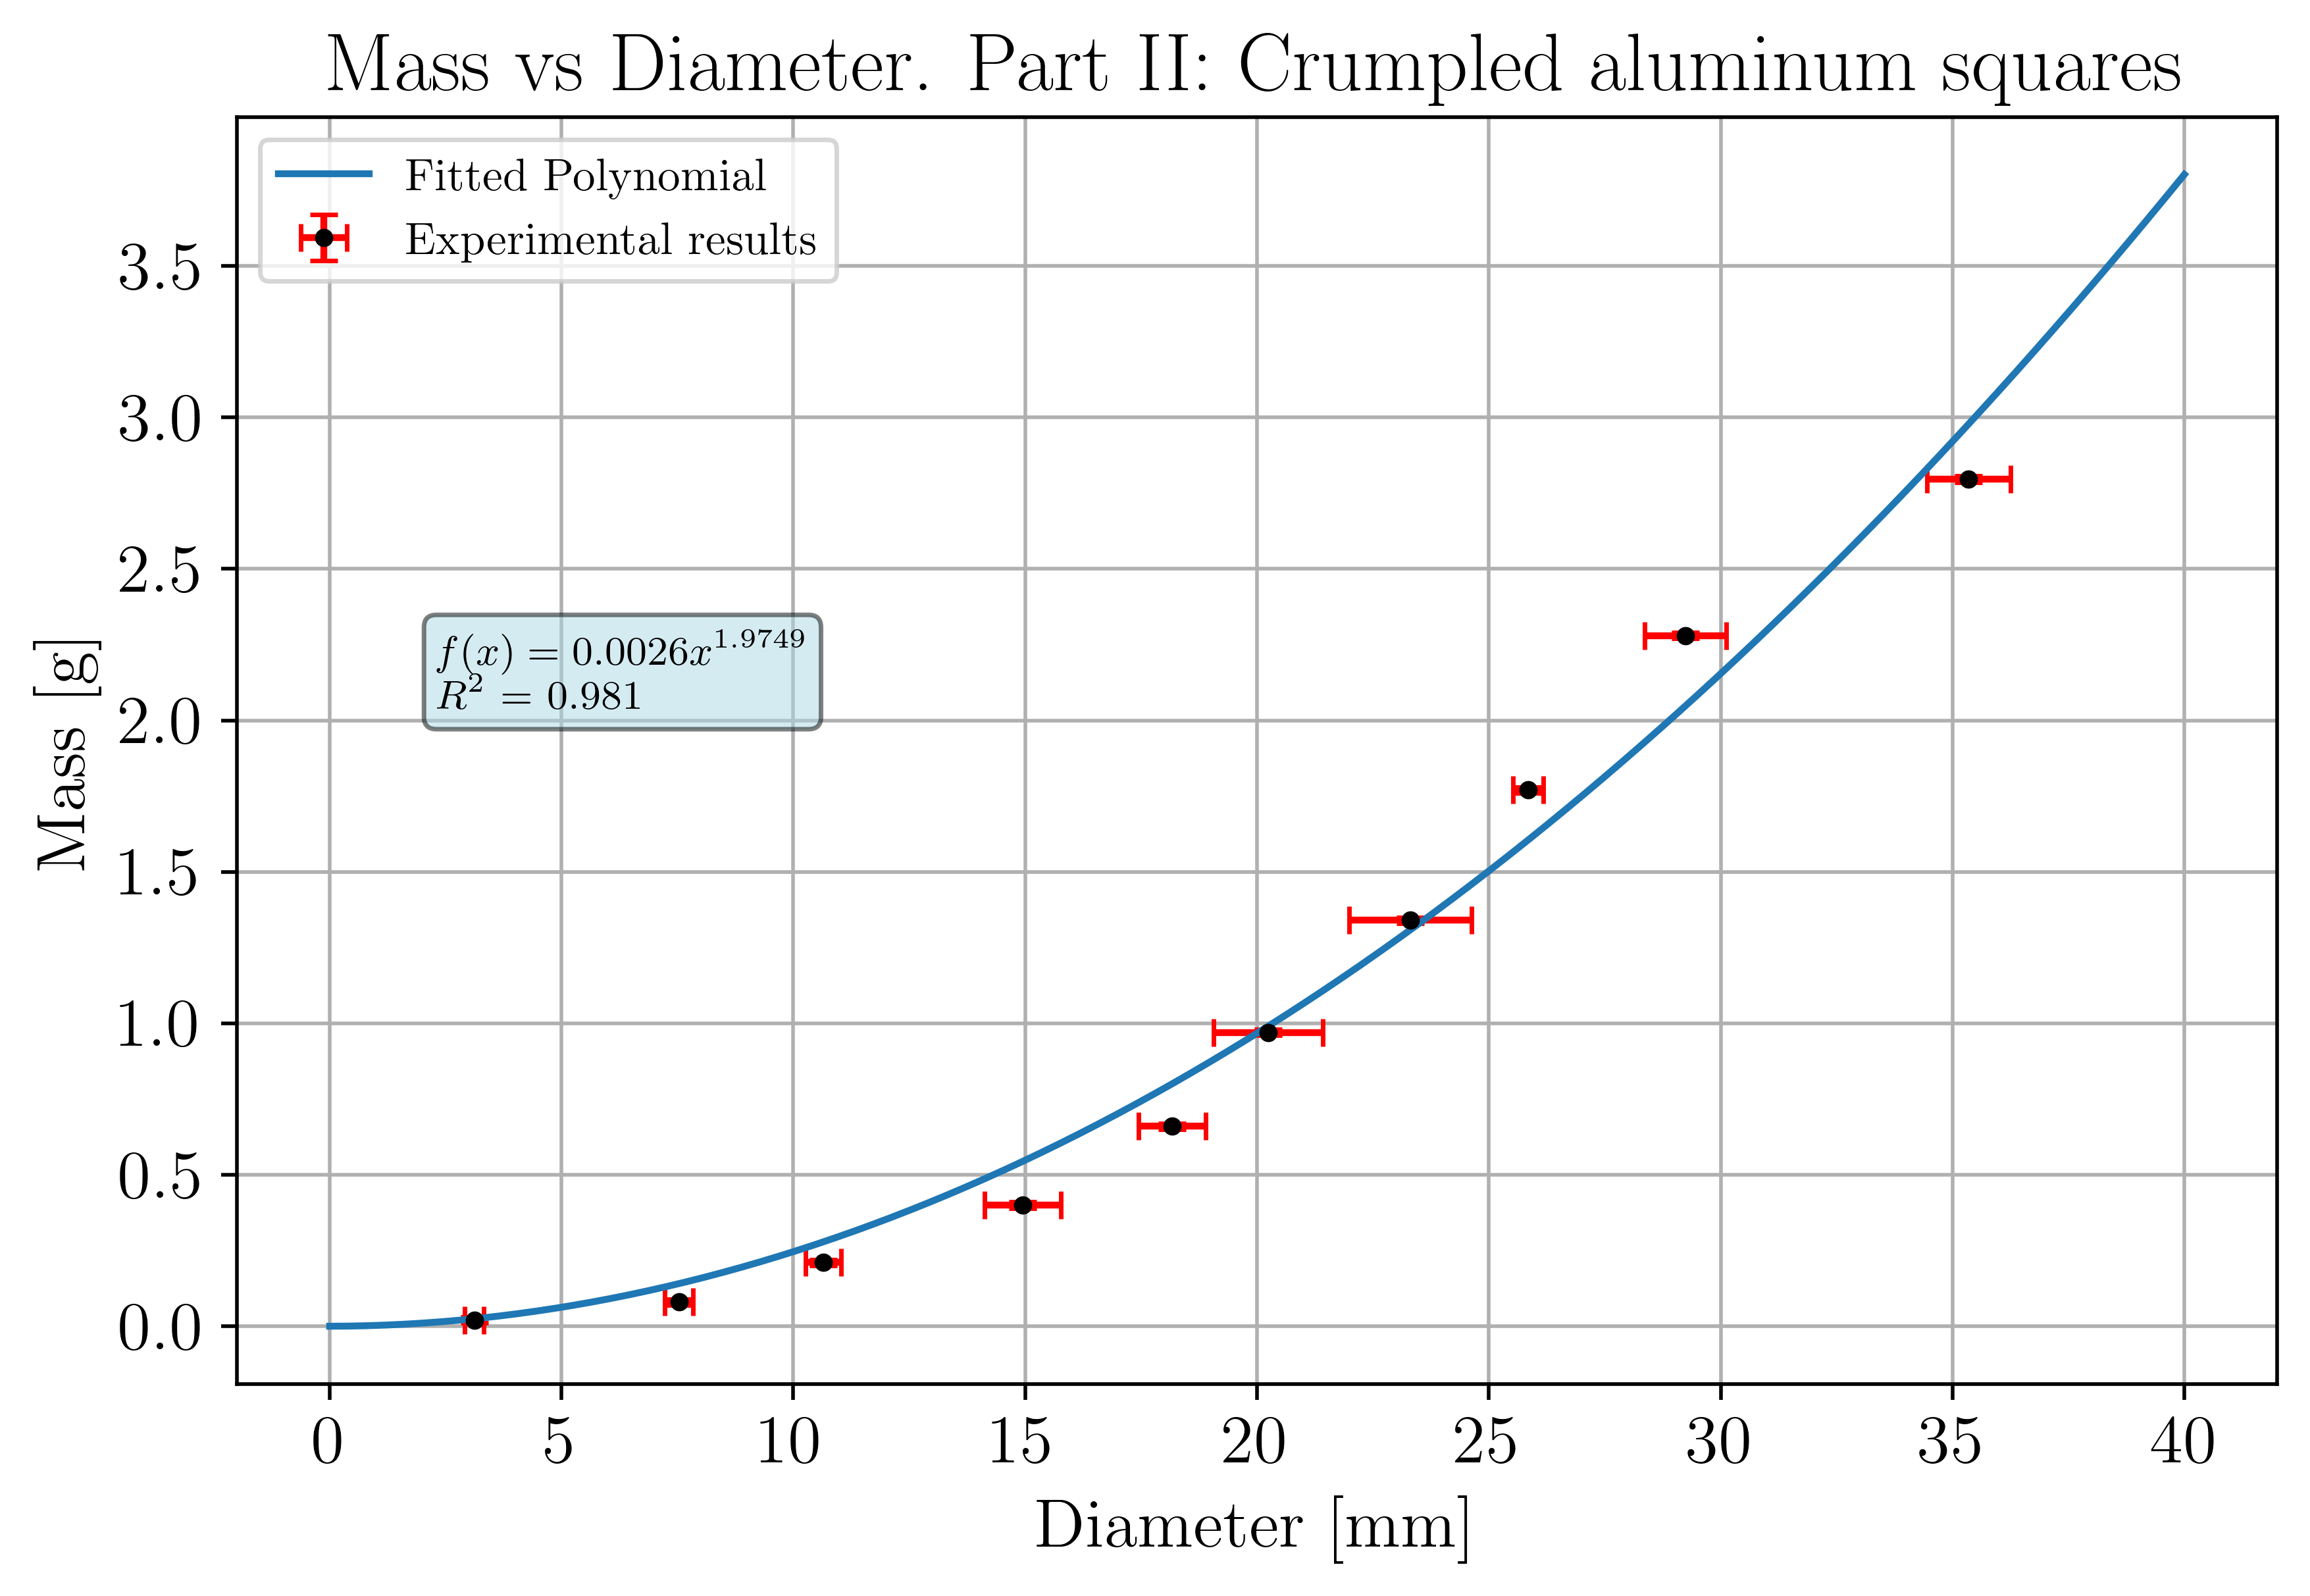
\includegraphics[width = 0.8\textwidth]{mass_vs_diameter.png}
    \caption{Mass vs Diameter of the Aluminum Balls. As expected, the data is well represented by a power law.}
    \label{fig:mass_vs_diameter}
\end{figure}

Finally, we compare the previous results with the ones obtained from the Least Squares method. The plot shown in Fig. (\ref{fig:ln_mass_vs_ln_diameter}) describes the relationship between the natural logarithm of the mass and the natural logarithm of the diameter of the aluminum balls.

\begin{figure}[h!]
    \centering
    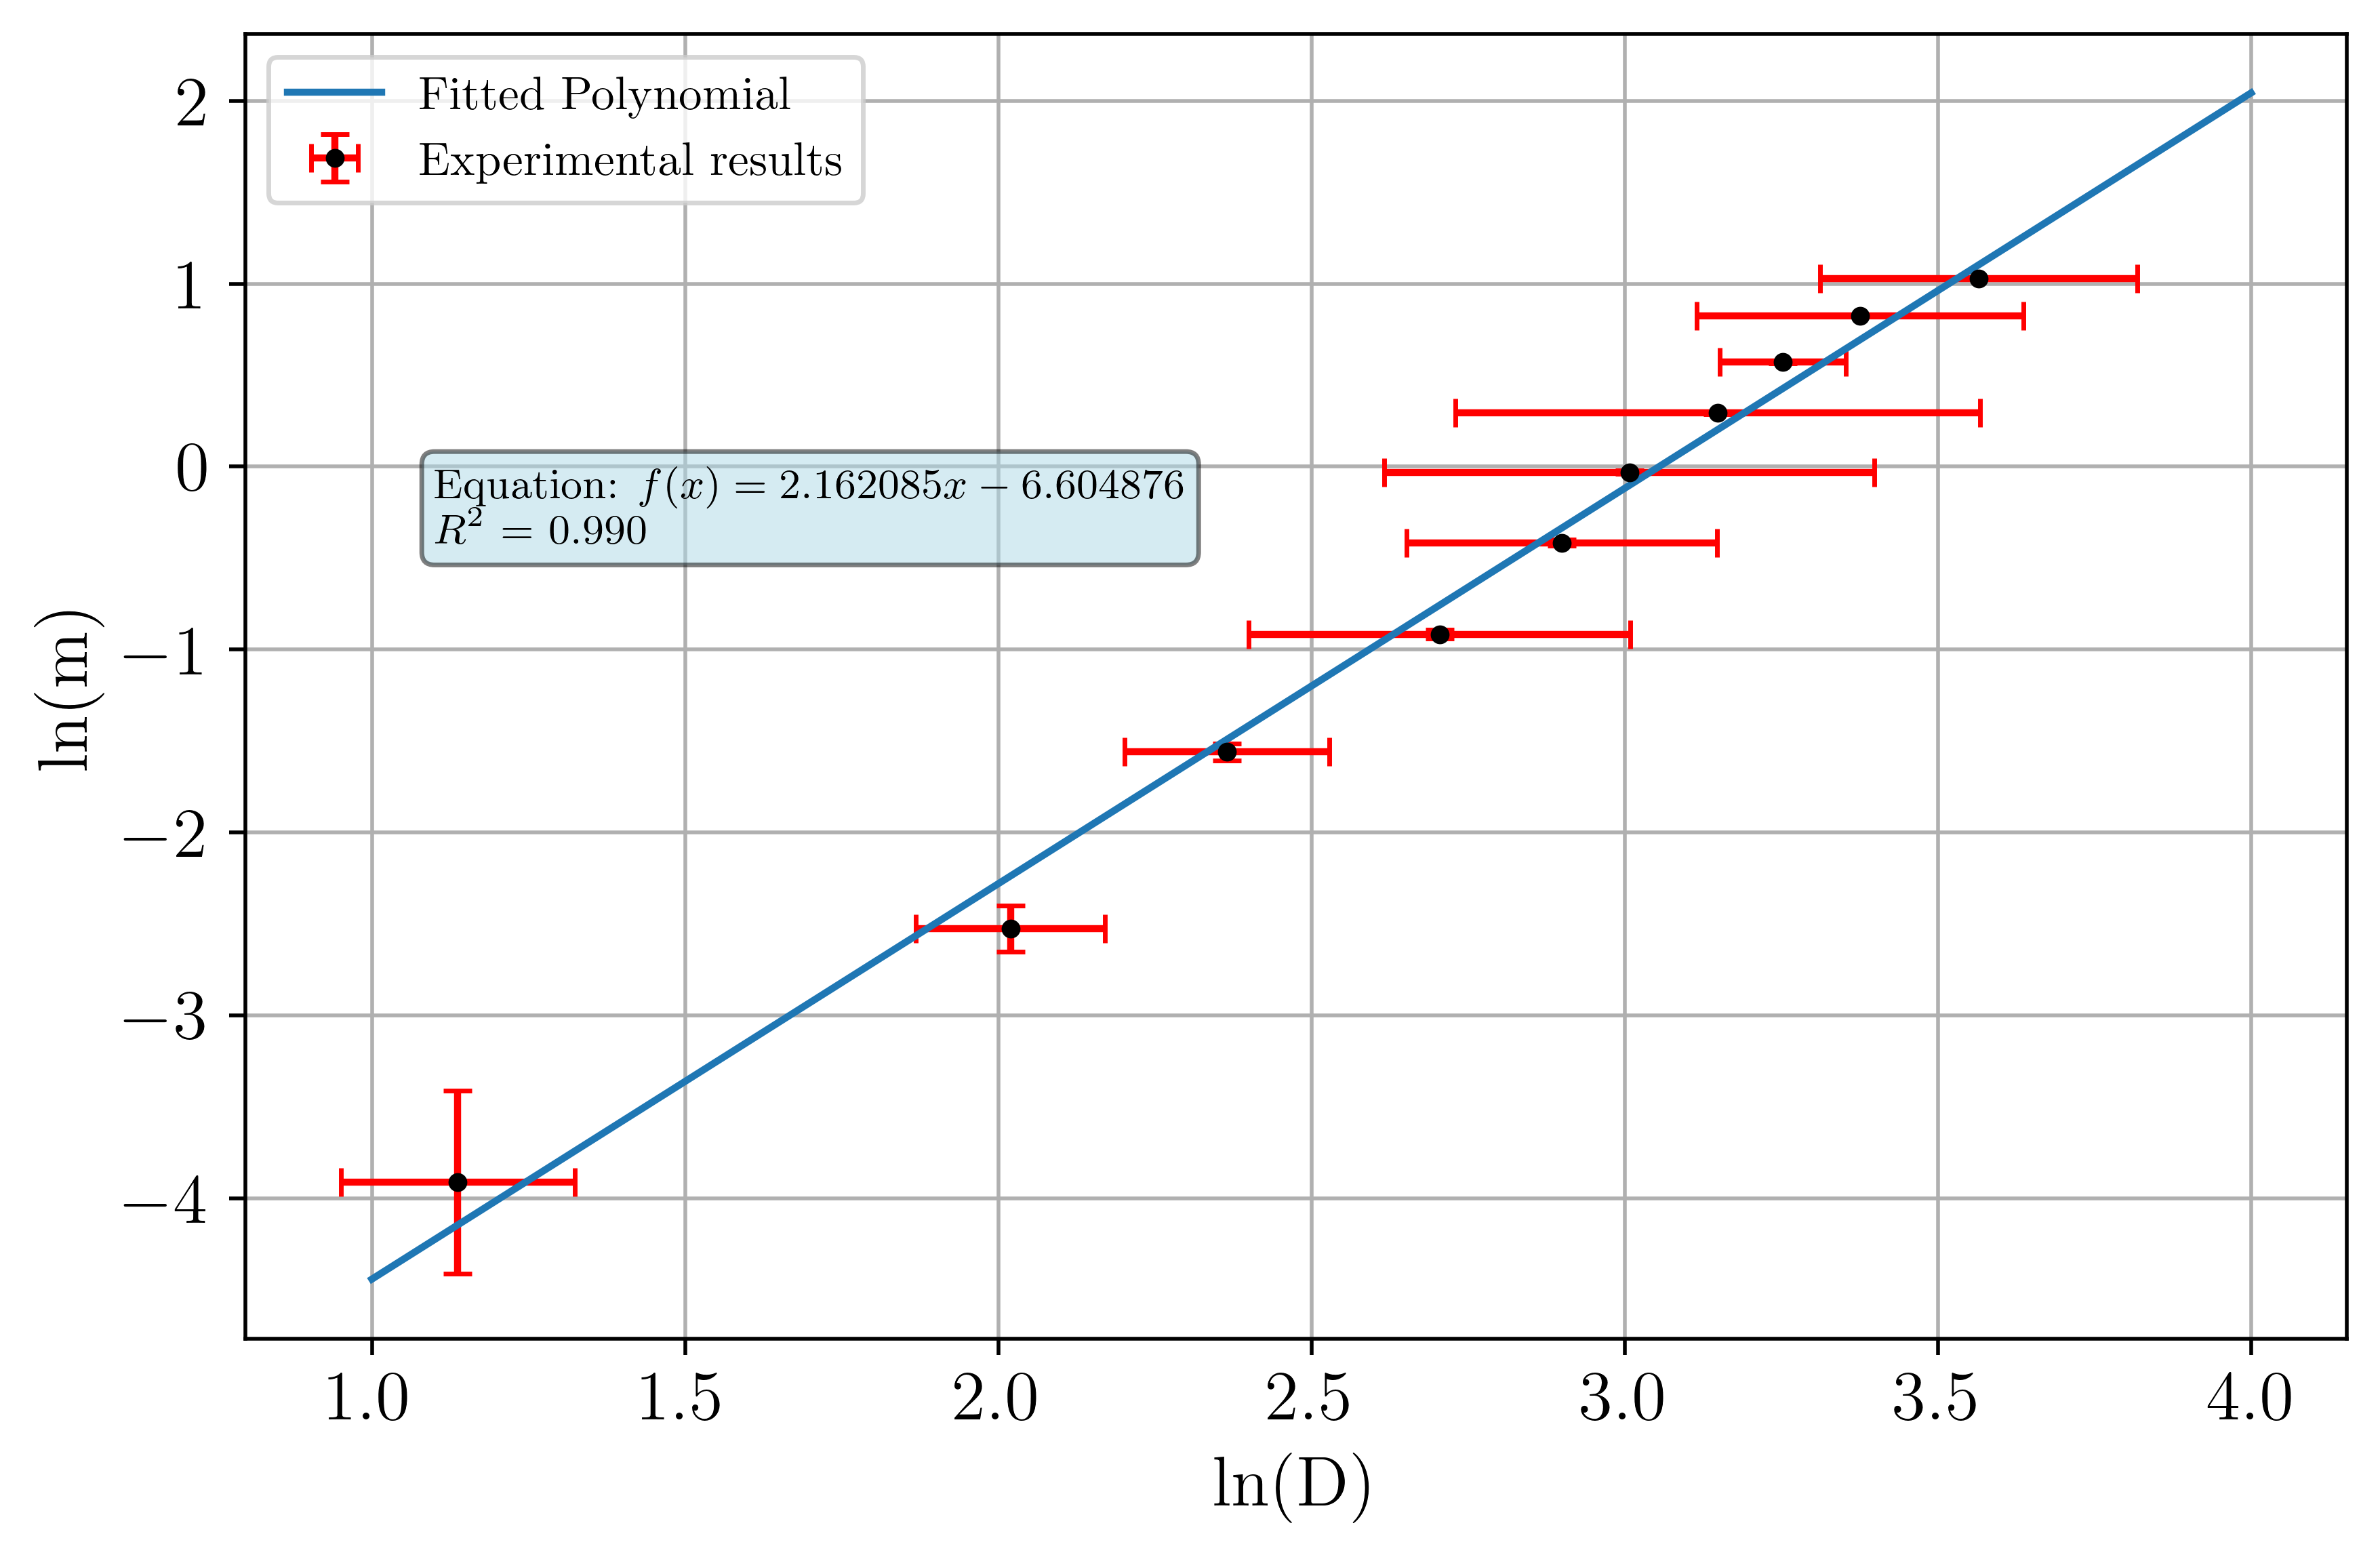
\includegraphics[width = 0.8\textwidth]{ln_mass_vs_ln_diameter.png}
    \caption{Natural logarithm of Mass vs Natural logarithm of Diameter of the Aluminum Balls. Alternative approach for the computation of the dimensionality parameters.}
    \label{fig:ln_mass_vs_ln_diameter}
\end{figure}

As before, we use the Least Square method to compute the parameters of the power law we are interested in. In Fig. (\ref{fig:ln_mass_vs_ln_diameter}), we show the linear law that best fits the data, whose parameters are $\ln(k) = -6.60 \pm 0.22$ and $\alpha = 2.16 \pm  0.08$. These results are closer to the ones expected and we consider them more reliable than the ones obtained from the previous method.
 
% Conclusion 
\section{Conclusion}\label{sec:conclusion}
The purpose of this experiment is to demonstrate that the fractal dimension of our aluminum tinfoil spheres, 
which are neither completely solid nor completely hollow, falls between 2 and 3.
Following the procedure outlined in (\ref{subsec:Experimental procedure}),
we measured the sides of the alluminum squares and then crumpled them into alluminum spheres.
All the collected data in shown in tables (\ref{tab:squares}) and (\ref{tab:balls}). 
Next, we analyzed the graphs (\ref{fig:mass_vs_length}), (\ref{fig:ln_mass_vs_ln_length}), (\ref{fig:mass_vs_diameter}), (\ref{fig:ln_mass_vs_ln_diameter}) 
initially applying a power law, followed by linear regression after linearizing Equation (\ref{eq:gen_fractal}).
Afterward, is it possible to compare te results obtained with the power law with those obtained from the linear regression.
% Appendix 
\section{Appendix}
Include supplementary information such as raw data, calculations, or additional graphs that are too detailed for the main report but are still relevant.

% References
\newpage
\printbibliography

\end{document}
